% Transcribed from blueprint/src/parts/05-price.tex.
\section{Exact or isotropic on a lattice, not both}
\label{ch:price}

Section~\ref{ch:matern} found a pyramid with the properties one would want on the continuum. The
\Matern{} pyramid is covariant under every dilation, its octave step is one implicit Euler step of
the heat equation, and its kernels are rotation invariant (Theorem~\ref{thm:matern-pyramid}). But a
pyramid is computed on a grid. This section asks how much of that survives there.

The first property wanted on a grid is exactness. A grid pyramid applies one array of weights, the
\emph{mask}, on the grid of every level, spread out by the factor $q$ from one level to the next. It
is exact when these steps are the octave steps of one family of kernels, continuous in scale and
covariant under $q$. The family need not be symmetric, though its mask is. Every step is still
infinitely divisible (Lemma~\ref{lem:steps-infinitely-divisible}), and the ladder fixes the kernels
at the knots (Lemma~\ref{lem:knot-data}). An exact pyramid also has a symmetric family through its
ladder, by Proposition~\ref{prop:ladder-knot-kernel}(2) as the proof of
Proposition~\ref{prop:exact-masks} uses it. To that family the results of Section~\ref{ch:pyramid}
on symmetric families apply. These are Proposition~\ref{prop:ladder-knot-kernel} and the
description of covariance under $q$ in Lemma~\ref{lem:discrete-covariance-levy}. In $d \ge 2$ the
results that assume isotropy do not apply. These are
the descriptions of the strata in Theorem~\ref{thm:lattice-strata} and the selection of
Section~\ref{ch:matern}. Without exactness, the steps of the pyramid are the octave steps of no
such family, and none of these results applies.

The second property is isotropy. A pyramid is isotropic when some kernel of its family at a
positive scale is rotation invariant. Smoothing by a rotation-invariant kernel commutes with
rotating the input, so smoothing by that kernel treats every orientation of an image alike. The
definition is deliberately weak, since one kernel at one positive scale suffices. That makes the
negative result below strong.

On a lattice in $\RR^d$, $d \ge 2$, the two cannot be had together. An exact grid pyramid whose
mask is carried by a lattice is never isotropic (Proposition~\ref{prop:grid-pyramid-not-isotropic}).
A pyramid on a lattice must give up one of them. If it keeps exactness, no kernel of its family at a
positive scale is rotation invariant. When the support of the mask spans $\RR^d$, each such kernel
has only finitely many orthogonal symmetries. If it gives up exactness, it gives up the family, and
with it the isotropy defined here, which is a property of the family. No mask other than
$\delta_0$ with an exponential moment, as every finite mask has, has a rotation-invariant refinable
law (Proposition~\ref{prop:no-isotropic-refinable-finite-mask}).

The reason lies in the jumps. Every step of a family continuous in scale is infinitely divisible
(Lemma~\ref{lem:steps-infinitely-divisible}). Its \Levy{} measure, as in
Section~\ref{ch:pyramid}, is the rate of its jumps of each size and direction. When the step is a
mask on a lattice, it has no Gaussian part and every jump is a lattice vector
(Lemma~\ref{lem:lattice-infinitely-divisible}). The kernel at a knot applies the mask at every finer
scale. So it too has no Gaussian part, it does jump, and its jumps are the lattice vectors shrunk
by the powers of $q$ (Proposition~\ref{prop:grid-pyramid-not-isotropic}(1)). That set is denser
than the lattice, but it is still countable. A rotation-invariant law that jumps by a vector $x$ at
a positive rate jumps at the same rate by every vector of the length of $x$. In $d \ge 2$ those
vectors form a sphere, which is uncountable, and a countable set cannot hold a sphere of such
atoms. On the line the sphere is the two points $\pm x$, and the obstruction is empty there.

Beyond the obstruction, the section says which masks give an exact pyramid and what the pyramid
algorithm computes with them.
\begin{itemize}
\item Section~\ref{sec:price-senses} separates three senses of the word \emph{exact} on a grid: for
a computation, for a family of kernels and for a pyramid. The obstruction is about the third.
\item Section~\ref{sec:price-obstruction} defines the exact grid pyramid and proves the
obstruction. Its example is the frame \Matern{} pyramid on the grid, whose mask samples the octave
step of the frame \Matern{} pyramid. It is exact in every dimension, and in $d \ge 2$ its octave
step fails the implicit-Euler principle on the grid as on the continuum.
\item Section~\ref{sec:price-masks} shows that a mask has an exact pyramid if and only if it is
infinitely divisible with a logarithmic moment, and that the resolvent masks of the discrete
Laplacians meet this criterion. It then follows an input through the levels of the computed
pyramid, shows that one level can create local maxima, and says what the pyramid algorithm returns.
\item Section~\ref{sec:discrete-helmholtz} constructs the resolvents of the $(2d+1)$-point and
nine-point Laplacians, which Sections~\ref{sec:price-senses} and~\ref{sec:price-masks} use as masks.
It reads independently of the rest of this section and may be read first.
\end{itemize}

Throughout, $\Gamma \subset \RR^d$ is a full-rank lattice: $h\ZZ^d$, or the hexagonal lattice in
the plane. For $c > 0$, $D_c\mu$ is the image of a measure $\mu$ under $x \mapsto cx$, as in
Definition~\ref{def:family-dimension-d}, so that $\widehat{D_c\mu}(\omega) = \widehat{\mu}(c\omega)$.
For $R \in \Orth(d)$, $D_R\mu$ is its image under $x \mapsto Rx$.

\subsection{Three senses of exact}
\label{sec:price-senses}

On a grid the word \emph{exact} is used for three different things. It is said of a computation
whose arrays are the kernels they stand for. It is said of a family of kernels when keeping every
$q$-th value of a member, and renormalizing, gives a member again. And it is said of a pyramid
whose ladder is that of a continuous covariant family. The three are easily confused, and a
negative result is only as strong as the sense it uses. So the senses are fixed first.

One convention holds for the whole section. A kernel on the grid $h\ZZ^d$ is a law
$w = \sum_{n \in \ZZ^d} w(n)\,\delta_{hn}$. Its weight at $hn$ is written $w(n)$ or $w(hn)$. Its
transform at the frequency $\omega$ is $\sum_n w(n)e^{ih\langle n, \omega\rangle}$, a function of
the grid frequency $\vartheta = h\omega$. Convolution on $h\ZZ^d$ is convolution of the weights on
$\ZZ^d$. A statement says which variable its transform takes, $\omega$ or $\vartheta$.

The second sense compares a family on a fine grid with the same family on a coarser one. That needs
a family defined on every grid by the same rule, which the next definition calls a grid family. Its
first kind is built from a discrete Laplacian. The $(2d+1)$-point Laplacian $\Delta_h$ on $h\ZZ^d$
is the usual second difference along each axis, and the nine-point Laplacian $\Delta_9$ on $h\ZZ^2$
also uses the four diagonal neighbours. The resolvent $\kappa_t$ is the kernel of the inverse of
$1 - t^2\Delta_h$, the grid counterpart of one implicit Euler step. It is the law of a geometric
number of steps of the simple random walk. Let $\sigma$ be the step of mass $1/(2d)$ at each
$\pm e_i$ of $\ZZ^d$, and $p := 2dt^2/(h^2 + 2dt^2)$. Then $\kappa_t = (1-p)\sum_{k \ge 0}p^k\sigma^{*k}$.
The nine-point resolvent $\kappa^9_t$ is $(1-p_9)\sum_{k \ge 0}p_9^k\sigma_9^{*k}$, with
$p_9 := 10t^2/(3h^2 + 10t^2)$ and the step $\sigma_9$ of mass $1/5$ at each $\pm e_i$ and $1/20$ at
each $\pm e_1 \pm e_2$ of $\ZZ^2$. These kernels are constructed in
Section~\ref{sec:discrete-helmholtz}, which may be read first.

% shared with blueprint def:grid-family
\begin{definition}[grid family]
\label{def:grid-family}

A \emph{grid family} on a lattice is one of the following families of kernels on that lattice.
\begin{enumerate}
\item For the $(2d+1)$-point Laplacian $\Delta_h$ on $h\ZZ^d$
(Proposition~\ref{prop:discrete-helmholtz}): the convolution powers $\kappa_t^{*\gamma}$, $t > 0$,
$\gamma \ge 1$ an integer, of its resolvents $\kappa_t$, the summable solutions of
$(1 - t^2\Delta_h)\kappa_t = \delta_0$. For the nine-point Laplacian $\Delta_9$ on $h\ZZ^2$
(Proposition~\ref{prop:nine-point-family}): the same, with $\Delta_9$ in place of $\Delta_h$.
\item For a mask $w$ on the lattice: its convolution powers $w^{*n}$, $n \ge 1$.
\end{enumerate}
\end{definition}

The list is closed on purpose. A family defined as the samples of continuum kernels is a grid
family only where it equals one of these. The sampled Laplace family on $h\ZZ$ is one, since it
equals the family of the three-point Laplacian (Proposition~\ref{prop:recursion-helmholtz}(2)).
Without the restriction, sense (ii) below could hold for a family only because it samples a
continuum family. The samples of an isotropic Gaussian on $h\ZZ^2$, subsampled by $q$, are the samples of the
same Gaussian on $qh\ZZ^2$. Read literally, they would be exact in sense (ii), and they are not a
grid family.

% shared with blueprint def:exact-senses
\begin{definition}[three senses of \emph{exact}]
\label{def:exact-senses}

The word \emph{exact} has three senses for a pyramid or a grid computation, each fixed by what it
is attached to.
\begin{enumerate}
\item A \emph{grid computation} is exact when the arrays it produces, in exact arithmetic, equal
the kernels they stand for. These are a lattice law itself, or a continuum kernel through its renormalized samples on the current grid, as each use of the sense names.
\item Let $q \ge 2$ be an integer. The \emph{subsample} of a member $\lambda$ of a grid family on
a lattice $\Gamma$ is its restriction to the coarser grid $q\Gamma$: on $h\ZZ^d$, the array
$m \mapsto \lambda(qhm)$ of every $q$-th value along each axis. It is exact when, renormalized to
mass one, it is a member of the same family on $q\Gamma$. For item (1) of
Definition~\ref{def:grid-family} that is a kernel $\kappa_\tau^{*\gamma}$ of the same stencil on
$q\Gamma$, of some range $\tau > 0$ and some index $\gamma \ge 1$. For item (2) it is a power
$(D_qw)^{*n}$, $n \ge 1$, of the same array on $q\Gamma$. The renormalizing constant is the mass
the subsample keeps, $C = \lambda(q\Gamma)$, which is required to be positive.
\item A \emph{grid pyramid} is exact when a continuous, discretely covariant hemigroup carries its
ladder (Definition~\ref{def:exact-grid-pyramid}).
\end{enumerate}
\end{definition}

Each sense is a property of a different object. Sense (i) is a property of an implementation. A
floating-point run equals the arrays of an exact computation up to rounding. An exact computation
still differs from the continuum kernels by aliasing, the difference between the renormalized
samples and the kernels themselves (Proposition~\ref{prop:sampled-laplace-exact}(3)). Aliasing
comes from sampling, so exactness in sense (i) does not remove it.
Proposition~\ref{prop:line-and-arrays}(2) is a statement in sense (i).

Sense (ii) is a property of a family. It describes smoothing by a member $\lambda$ on the fine grid
followed by keeping every $q$-th value. The impulse response of the two operations together is the
subsample of $\lambda$, so the averaging over neighbouring fine values is already in $\lambda$. The
constant $C$ is below $1$ whenever $\lambda$ charges a point off the coarse grid. This paper makes
one statement in sense (ii), on the line. The subsample of a sampled Laplace kernel is the kernel
of the same range on the coarser grid (Proposition~\ref{prop:sampled-laplace-exact}(2)). The sense
is fixed here to keep the subsample of a family apart from the ladder of a mask. The results of
this section are about the ladder. In $d \ge 2$, which members of the discrete Helmholtz family
have an exact subsample is left to further work.
% TODO(module computation): cite prop:helmholtz-subsampling when released

Sense (iii) is a property of a mask and a ratio, made precise by
Definition~\ref{def:exact-grid-pyramid} in the next subsection. It is the sense of every statement
that calls a pyramid exact in dimension $d \ge 2$, and of \emph{exact} in every sentence that
carries Proposition~\ref{prop:grid-pyramid-not-isotropic}.

The phrase \emph{exact cascade} (Propositions~\ref{prop:discrete-helmholtz}(2)
and~\ref{prop:nine-point-family}(2)) names none of the three. It is used for a family on one grid
in which the step between any two members is again a probability kernel on that grid, so that
members and steps satisfy the hemigroup relation exactly.

\subsection{The exact grid pyramid, and why on a lattice it is not isotropic}
\label{sec:price-obstruction}

This subsection makes sense (iii) precise and proves that, in $d \ge 2$, it excludes isotropy. The
definition requires a family of laws on $\RR^d$, continuous in scale and covariant under $q$, whose
octave step from scale $1$ to scale $q$ is the mask. Only that step is tied to the lattice, and the
kernels of the family need not live on it. The proof shows that they still inherit enough of the
lattice to lose rotation invariance. Its tool is Lemma~\ref{lem:lattice-infinitely-divisible},
which puts the jumps of an infinitely divisible law carried by a lattice on that lattice.

% shared with blueprint def:exact-grid-pyramid
\begin{definition}[exact grid pyramid in $\RR^d$]
\label{def:exact-grid-pyramid}

Let $d \ge 1$, let $\Gamma \subset \RR^d$ be a full-rank lattice, let $q > 1$, and let $w$ be a
symmetric probability law on $\Gamma$ with $w \ne \delta_0$, the \emph{mask}. The
\emph{grid pyramid} of $(w, q)$ on $\Gamma$ is its \emph{ladder}, the sequence of octave steps
$w_n := D_{q^n}w$, $n \in \ZZ$, the same array applied on the grid $q^n\Gamma$ at every level. It is
\textbf{exact} if some family $(\mu_{s,t})_{0 \le s \le t}$ of probability laws on $\RR^d$ carries
it, in the sense that
\begin{enumerate}
\item[(a)] $\mu_{s,t} * \mu_{t,u} = \mu_{s,u}$ for $s \le t \le u$, and $\mu_{t,t} = \delta_0$
(hemigroup);
\item[(b)] $(s,t) \mapsto \mu_{s,t}$ is weakly continuous on $\{0 \le s \le t\}$ (continuity in
scale);
\item[(c)] $\mu_{qs,qt} = D_q\mu_{s,t}$ for $0 \le s \le t$ (discrete covariance);
\item[(d)] $\mu_{1,q} = w$.
\end{enumerate}
A carrying family need not be symmetric and need not have (ND). The \emph{kernels} are $\mu_t := \mu_{0,t}$. The \emph{knots} are the scales $q^n$, the levels of
the pyramid, and the $\mu_{q^n}$ are the \emph{knot kernels}, all dilates of $\mu_1$ by (c). The
pyramid is \emph{isotropic} if some kernel $\mu_t$ with $t > 0$ is rotation invariant, that is
$D_R\mu_t = \mu_t$ for every $R \in \mathrm{SO}(d)$. $\mathrm{SO}(1)$ is trivial, so at $d = 1$ every pyramid
is isotropic in this sense.
For every symmetric probability law $w \ne \delta_0$ on $\RR^d$, carried by a lattice or not, the
\emph{ladder} of $(w, q)$ is the sequence $D_{q^n}w$, $n \in \ZZ$. It is \textbf{exact}, the
\emph{exact ladder of $(w, q)$}, if some family of probability laws on $\RR^d$ has (a)--(d).
Kernels, knots, knot kernels and isotropy are read as above. For a mask on $\Gamma$ the ladder is
the grid pyramid, and it is exact exactly when the grid pyramid is. The words \emph{grid pyramid}
are kept for a mask carried by a lattice.
\end{definition}

By (c) and (d), $\mu_{q^n, q^{n+1}} = D_{q^n}\mu_{1,q} = w_n$. So a family that meets one octave
step meets the whole ladder, as in Definition~\ref{def:grid-pyramid-line}. Conditions (a)--(c) are
what the axioms of \prog{iso v0.1}{Def.~3.2, p.~11} say about the laws of the operators
$\Phi_{s,t}$, with three changes. Rotation invariance, (I3) there, is dropped. Covariance is
required at the one ratio $q$, with the scale multiplied by $q$, where (I4) allows any increasing
relabelling. Nondegeneracy, (ND) there, is required only of the octave step, by $w \ne \delta_0$. A weaker notion would require only the knot relation
$D_q\mu_1 = \mu_1 * w$ of Section~\ref{sec:pyramid-bounded}. The continuity (b) is required instead
for two reasons. The knot relation alone admits finite masks, the binomial mask among them
(Proposition~\ref{prop:binomial-knot-relation}). For some masks of infinite support it also admits
rotation-invariant laws, so without (b) the obstruction to isotropy below would fail
(Proposition~\ref{prop:band-limited-refinable-mask}).

The knot kernel of a carrying family is fixed by the mask, whatever the family does between
the knots. Only the mask is assumed symmetric, not the family, so the next lemma is not a case of
Proposition~\ref{prop:ladder-knot-kernel}(1).

% shared with blueprint lem:knot-data
\begin{lemma}[the knot kernel of a carrying family]
\label{lem:knot-data}

Let $d \ge 1$ and $q > 1$, let $w$ be a symmetric probability law on $\RR^d$, and let a family
$(\mu_{s,t})_{0 \le s \le t}$ of probability laws on $\RR^d$ have (a)--(d) of
Definition~\ref{def:exact-grid-pyramid}. Then
\[
  \widehat{\mu_1}(\omega) = \lim_{M \to \infty}\prod_{m=1}^M\widehat{w}\bigl(q^{-m}\omega\bigr),
  \qquad \omega \in \RR^d,
\]
and $\mu_1$ is symmetric. If $w$ has the \Levy{} data $(A_w, \nu_w)$, then $\mu_1$ has the data
$\bigl(A_w/(q^2 - 1), \nu^*\bigr)$, with $\nu^* := \sum_{m \ge 1}D_{q^{-m}}\nu_w$.
\end{lemma}

\begin{proof}
\emph{The product.} The law $\mu_1 = \mu_{0,1}$ is infinitely divisible, by
Lemma~\ref{lem:steps-infinitely-divisible}. Its (I1) is (a), convolution being commutative, and its
(I2) follows from (b), as $x \mapsto e^{i\langle\omega, x\rangle}$ is bounded and continuous. By
(a), (c) and (d), $D_q\mu_1 = \mu_{0,q} = \mu_{0,1} * \mu_{1,q} = \mu_1 * w$, so
$\widehat{\mu_1}(q\omega) = \widehat{w}(\omega)\widehat{\mu_1}(\omega)$, and by induction
\[
\widehat{\mu_1}(\omega) = \widehat{\mu_1}(q^{-M}\omega)\prod_{m=1}^M\widehat{w}(q^{-m}\omega),
\qquad M \ge 1 .
\]
The transform of $\mu_1$ has no zero (\ledger{A40}). As $M \to \infty$,
$\widehat{\mu_1}(q^{-M}\omega) \to \widehat{\mu_1}(0) = 1$ by continuity of the transform, so the
partial products $\widehat{\mu_1}(\omega)/\widehat{\mu_1}(q^{-M}\omega)$ converge to
$\widehat{\mu_1}(\omega)$ at every $\omega$.

\emph{Symmetry.} The transform of the symmetric law $w$ is real, so $\widehat{\mu_1}$ is a limit of
products of real numbers, and it is real. The reflection of $\mu_1$ has the conjugate transform,
which is the same, so $\mu_1$ is symmetric.

\emph{The data.} Let $w$ have the data $(A_w, \nu_w)$. Being symmetric and infinitely divisible,
$\mu_1$ has data $(A_1, \nu_1)$, by Lemma~\ref{lem:symmetric-levy-khintchine}. The law $D_q\mu_1$
has the data $(q^2A_1, D_q\nu_1)$, by the substitution $y = qx$ in the exponent. The law
$\mu_1 * w$ has the data $(A_1 + A_w, \nu_1 + \nu_w)$, since exponents add. They are one law, so
uniqueness gives $q^2A_1 = A_1 + A_w$, that is $A_1 = A_w/(q^2 - 1)$, and
$D_q\nu_1 = \nu_w + \nu_1$. Applying $D_{q^{-1}}$ $M$ times,
\[
\nu_1 = \sum_{m=1}^M D_{q^{-m}}\nu_w + D_{q^{-M}}\nu_1 .
\]
For a Borel set $B \subseteq \{|x| > \varepsilon\}$, $\varepsilon > 0$, the last term is
$\nu_1(q^MB) \le \nu_1(\{|x| > q^M\varepsilon\})$, which tends to $0$, a \Levy{} measure being
finite off every neighbourhood of $0$. So $\nu_1$ and $\nu^*$ agree off every ball about $0$, and
neither charges $0$: $\nu_1 = \nu^*$, the argument of Proposition~\ref{prop:ladder-knot-kernel}(1).

Every step is machine-checked, and the cited facts are \ledger{A40}, with \ledger{A41} and
\ledger{A39} through the lemmas used.
\end{proof}

Conditions (a)--(c) allow isotropic families, since the isotropic \Matern{} pyramid of
Theorem~\ref{thm:matern-pyramid} satisfies them. What excludes isotropy is (d), the one condition
about the grid, together with the continuity (b). The next proposition follows the jumps, as
sketched at the start of this section. Clause (1) shows that the mask is infinitely divisible with
its jumps on $\Gamma$, and that the knot kernel applies the mask at every finer scale, so that its
jumps lie on a countable set $\Gamma_q$. Clause (2) draws the conclusion. Clause (3) shows that the
definition is not empty: exact grid pyramids on a lattice exist in every dimension.

% shared with blueprint prop:grid-pyramid-not-isotropic
\begin{proposition}[no exact grid pyramid on a lattice is isotropic in $d \ge 2$]
\label{prop:grid-pyramid-not-isotropic}

Let $(w, q)$ be an exact grid pyramid on the lattice $\Gamma \subset \RR^d$, carried by the family
$(\mu_{s,t})$, and put $\Gamma_q := \bigcup_{k \in \ZZ}q^k\Gamma$, a countable set, which for
integer $q$ and $\Gamma = h\ZZ^d$ is $h\ZZ[1/q]^d$.
\begin{enumerate}
\item \emph{(The covariant kernel.)} The mask $w$ is infinitely divisible: it is the compound
Poisson law with a finite \Levy{} measure $\nu_w \ne 0$ carried by $\Gamma \setminus \{0\}$. The
knot kernel is determined by the mask,
\begin{equation}\label{eq:knot-product}
\mu_1 = \lim_{M \to \infty} D_{q^{-1}}w * D_{q^{-2}}w * \dots * D_{q^{-M}}w, \qquad
\widehat{\mu_1}(\omega) = \prod_{m \ge 1}\widehat{w}\bigl(q^{-m}\omega\bigr).
\end{equation}
Every kernel $\mu_t$, $t > 0$, is infinitely divisible with no Gaussian part and a nonzero \Levy{}
measure $\nu_t$ carried by $\Gamma_q$, and at the knots
$\nu_{q^n} = \sum_{m \ge 1} D_{q^{n-m}}\nu_w$.
\item \emph{(No isotropy.)} If $d \ge 2$, no kernel $\mu_t$, $t > 0$, is rotation invariant. If
moreover $\operatorname{supp} w$ spans $\RR^d$, then for every $t > 0$ the group
$\{R \in \Orth(d) : D_R\mu_t = \mu_t\}$ is finite.
\item \emph{(Existence: the frame \Matern{} pyramid on the grid.)} Exact grid pyramids on a lattice exist in every dimension. Clause (3) does not assume the opening hypotheses. For $0 < a < 1$ let $\lambda^{\mathrm L}_a(hn) := \tfrac{1-a}{1+a}a^{|n|}$, $n \in \ZZ$,
be the sampled Laplace mask on $h\ZZ$: the kernel $\lambda_t$ of
Proposition~\ref{prop:sampled-laplace-exact} at $a = a_t = e^{-h/t}$, written in its ratio $a$. For
every $q > 1$ the grid pyramid of $((\lambda^{\mathrm L}_a)^{\otimes d}, q)$ on $h\ZZ^d$ is exact.
Its knot kernel is
\[
\widehat{\mu_1}(\omega) = \prod_{i=1}^d\prod_{m \ge 1}\Bigl[1 + \frac{2a}{(1-a)^2}
\bigl(1 - \cos(q^{-m}h\omega_i)\bigr)\Bigr]^{-1},
\]
and its \Levy{} measure
\begin{equation}\label{eq:frame-levy}
\nu_1 = \sum_{i=1}^{d}\sum_{m \ge 1}\sum_{n \ne 0}\frac{a^{|n|}}{|n|}\,\delta_{nhq^{-m}e_i}
\end{equation}
is carried by the coordinate axes. The symmetry group of every knot kernel is the hyperoctahedral
group of signed permutations of the axes.
\end{enumerate}
\end{proposition}

\begin{proof}
Throughout, an infinitely divisible law has the generating triplet $(A^{\mathrm S}, \nu, \gamma)$ of
\ledger{A39}(i), unique by \ledger{A39}(ii). Triplets add under convolution, since the transform of
a convolution is the product of the transforms and the exponents of the formula of \ledger{A39}(i)
add. A symmetric infinitely divisible law has unique \Levy{} data $(A, \nu)$ and the triplet
$(2A, \nu, 0)$, by Lemma~\ref{lem:symmetric-levy-khintchine}. The data of a dilate $D_c\mu$, $c \ne 0$, are $(c^2A, D_c\nu)$, by the
substitution $y = cx$ in the exponent. The mask is a probability law other than $\delta_0$, so
$d \ge 1$: on $\RR^0$ every law is $\delta_0$.

(1) \emph{Every $\mu_{s,t}$ is infinitely divisible}, by
Lemma~\ref{lem:steps-infinitely-divisible}. Its (I1) is (a), convolution being commutative, and its
(I2) follows from (b), as $x \mapsto e^{i\langle\omega, x\rangle}$ is bounded and continuous.

\emph{The mask.} $w = \mu_{1,q}$ is infinitely divisible, symmetric and carried by $\Gamma$. It has
data $(A_w, \nu_w)$, so the triplet $(2A_w, \nu_w, 0)$, and by
Lemma~\ref{lem:lattice-infinitely-divisible}, applied to that triplet, $A_w = 0$ and the \Levy{}
measure $\nu_w$ is finite and carried by $\Gamma \setminus \{0\}$. So
$\widehat{w} = e^{-\psi_w}$ with $\psi_w(\omega) := \int(1 - \cos\langle\omega, x\rangle)\,
\nu_w(dx)$, which is the transform of the compound Poisson law
$e^{-\nu_w(\RR^d)}\sum_{k \ge 0}\nu_w^{*k}/k!$. So $w$ is that law. Finally $\nu_w \ne 0$, since
$w \ne \delta_0$.

\emph{The product formula.} By Lemma~\ref{lem:knot-data}, the partial products
$\prod_{m=1}^M\widehat{w}(q^{-m}\omega)$ converge to $\widehat{\mu_1}(\omega)$ at every $\omega$.
They are the transforms of the partial convolutions $D_{q^{-1}}w * \dots * D_{q^{-M}}w$, which
therefore converge weakly to $\mu_1$ by L\'evy's continuity theorem. This is
(\ref{eq:knot-product}).

\emph{\Levy{} data of the knot kernel.} By the same lemma, $\mu_1$ is symmetric with the data
$(A_w/(q^2 - 1), \nu^*) = (0, \nu^*)$, as $A_w = 0$, where $\nu^* := \sum_{m \ge 1}D_{q^{-m}}\nu_w$.
Write $\nu_1 := \nu^*$. This measure is carried by $\bigcup_{m \ge 1}q^{-m}\Gamma$, and $\mu_1$ has
no Gaussian part.

\emph{All kernels.} By (c), $\mu_{q^n} = D_{q^n}\mu_1$, whose data are $(0, D_{q^n}\nu_1)$, and
$D_{q^n}\nu_1 = \sum_{m \ge 1}D_{q^{n-m}}\nu_w$, the formula at the knots. Now let $t > 0$ and
choose $n$ with $q^n \le t < q^{n+1}$. By (a), $\mu_{q^{n+1}} = \mu_t * \mu_{t,q^{n+1}}$ and
$\mu_t = \mu_{q^n} * \mu_{q^n,t}$, all four factors infinitely divisible. Triplets add. The Gaussian
parts of $\mu_t$ and $\mu_{t,q^{n+1}}$ are positive semidefinite and sum to $0$, so both vanish.
The \Levy{} measures give $D_{q^n}\nu_1 \le \nu_t \le D_{q^{n+1}}\nu_1$. The upper bound puts
$\nu_t$ on $\bigcup_{m \ge 1}q^{n+1-m}\Gamma \subseteq \Gamma_q$. The lower bound makes it nonzero,
as $D_{q^n}\nu_1 \ge D_{q^{n-1}}\nu_w \ne 0$. The set $\Gamma_q$ is countable, a countable union of
images of the lattice, which is countable as a discrete subset of $\RR^d$. For $\Gamma = h\ZZ^d$ and
integer $q$, a point $q^khm$, $m \in \ZZ^d$, with $k \ge 0$ is $h(q^km) \in h\ZZ[1/q]^d$, and with
$k = -j < 0$ it is $h\,(m/q^j) \in h\ZZ[1/q]^d$. Conversely, a point of $h\ZZ[1/q]^d$ is $h\,m/q^j$
for some $m \in \ZZ^d$ and $j \ge 0$, a common denominator of its coordinates, and this is
$q^{-j}(hm) \in q^{-j}\Gamma$. This is the description of $\Gamma_q$ in the statement.

(2) Let $t > 0$ and $R \in \Orth(d)$ with $D_R\mu_t = \mu_t$. By \ledger{A42} with $U = R$,
the \Levy{} measure of $D_R\mu_t$ is $R_*\nu_t$, as $R$ maps only $0$ to $0$, so uniqueness gives
$R_*\nu_t = \nu_t$, and $\nu_t(\{Rx\}) = \nu_t(\{x\})$ for every $x$. By (1), $\nu_t \ne 0$ is
carried by the countable set $\Gamma_q$, so it has an atom $x$, and $x \ne 0$. Suppose $\mu_t$ is
invariant under $\mathrm{SO}(d)$ and $d \ge 2$. For every $y$ with $|y| = |x|$ some
$R \in \mathrm{SO}(d)$ has $Rx = y$. If $y = x$, take $R = I$. Otherwise the reflection in the
hyperplane orthogonal to $x - y$ maps $x$ to $y$, as $|x| = |y|$, and it is followed by the
reflection in a hyperplane containing $y$, which exists as $d \ge 2$, to make the determinant $+1$. So every point of the sphere $\{|y| = |x|\}$ is an atom
of $\nu_t$, and an atom of $\nu_t$ lies in $\Gamma_q$. But the sphere is uncountable: the points
$|x|\,(e_1 + se_2)/|e_1 + se_2|$, $s \in \RR$, lie on it and are distinct, the ratio of their second
coordinate to their first being $s$. This contradiction proves the first sentence.

For the finite group, let $V$ be the span of the atoms of $\nu_w$. The measure $\nu_w$ is carried
by the countable set $\Gamma$, and its points outside $V$ carry no mass, so $\nu_w(\RR^d \setminus
V) = 0$. For $\eta$ orthogonal to $V$, $\langle\eta, x\rangle = 0$ for $\nu_w$-almost every $x$, so
$\widehat{w}(\eta) = e^{-\psi_w(\eta)} = 1$. Then $\cos\langle\eta, x\rangle = 1$ for $w$-almost
every $x$, and the same at $\eta/k$ for every integer $k \ge 1$ forces $\langle\eta, x\rangle = 0$
for $w$-almost every $x$. So $w$ is carried by the orthogonal complement of $V^\perp$, which is $V$,
and every atom of $w$ lies in $V$. If the support of $w$, its set of atoms, spans $\RR^d$, so does
$V$, and some atoms $b_1, \dots, b_d$ of $\nu_w$ form a basis. With $n$ as in (1),
$\nu_t \ge D_{q^n}\nu_1 \ge D_{q^{n-1}}\nu_w$, so the points $x_i := q^{n-1}b_i$ are atoms of
$\nu_t$, and they form a basis. For each $i$ let $Y_i$ be the set of points $y$ with
$|y| = |x_i|$ and $\nu_t(\{y\}) \ge \nu_t(\{x_i\})$. It is finite, because
$\nu_t(\{|y| > |x_i|/2\}) < \infty$ and each point of $Y_i$ carries at least the mass
$\nu_t(\{x_i\}) > 0$. A symmetry $R$ is orthogonal and has $\nu_t(\{Rx_i\}) = \nu_t(\{x_i\})$, so
$Rx_i \in Y_i$. A linear map is determined by its values on a basis, so the group has at most
$\prod_i|Y_i|$ elements.

(3) \emph{The mask on the line.} The proof of
Proposition~\ref{prop:grid-pyramids-infinitely-divisible}(4) sums the transform of
$\lambda^{\mathrm L}_a$ as two geometric series and expands $\log|1 - ae^{ih\omega}|^2$, which gives
\[
\widehat{\lambda^{\mathrm L}_a}(\omega) = \frac{(1-a)^2}{1 - 2a\cos h\omega + a^2}
= \frac{1}{1 + \frac{2a}{(1-a)^2}\bigl(1 - \cos h\omega\bigr)}
= \exp\Bigl(-\int(1 - \cos\omega v)\,\varpi(dv)\Bigr),
\]
with the finite folded \Levy{} measure $\varpi := \sum_{k \ge 1}\tfrac{2a^k}{k}\delta_{kh}$. Its
symmetric form $\varpi_s := \tfrac12\bigl(\varpi + \varpi(-\,\cdot)\bigr) =
\sum_{n \ne 0}\tfrac{a^{|n|}}{|n|}\delta_{nh}$ has the same integral of $1 - \cos\omega v$.

\emph{The mask in $\RR^d$.} Let $w := (\lambda^{\mathrm L}_a)^{\otimes d}$ and
$\nu_w := \sum_i(\iota_i)_*\varpi_s$, with $\iota_i(v) := ve_i$. The transform of a product law is
the product of the transforms of its factors, so
\[
\widehat{w}(\omega) = \prod_{i=1}^d\widehat{\lambda^{\mathrm L}_a}(\omega_i)
= \exp\Bigl(-\sum_{i=1}^d\int(1 - \cos\omega_iv)\,\varpi_s(dv)\Bigr)
= \exp\Bigl(-\int(1 - \cos\langle\omega, x\rangle)\,\nu_w(dx)\Bigr),
\]
and $\nu_w$ is finite, symmetric, without atom at $0$. So $w$ has the data $(0, \nu_w)$. It is a
mask on $h\ZZ^d$: a probability law; symmetric, since its transform is real; carried by
$h\ZZ^d$, since each coordinate is carried by $h\ZZ$; and not $\delta_0$, since $\nu_w \ne 0$ and
$\delta_0$ has the data $(0, 0)$.

\emph{Exactness.} Since $\log_+ x \le x$ for $x \ge 0$,
\[
\int\log_+|x|\,\nu_w(dx) = d\sum_{k \ge 1}\frac{2a^k}{k}\log_+(kh)
\le 2dh\sum_{k \ge 1}a^k < \infty .
\]
So Proposition~\ref{prop:ladder-knot-kernel}(2) gives a symmetric $q$-covariant family with
$S_qt = qt$ and $\mu_{1,q} = w$. Its cascade (I1) is (a), convolution being commutative; its
continuity (I2) of the transforms gives (b) by \Levy's continuity theorem; and its covariance at
$q$ with $S_qt = qt$ is (c). So the grid pyramid of $(w, q)$ is exact, for every $q > 1$.

\emph{Every family carrying it.} By (1), the knot kernel is (\ref{eq:knot-product}), and its
factors are
$\widehat{w}(q^{-m}\omega) = \prod_i\bigl[1 + 2a(1-a)^{-2}\bigl(1 - \cos(q^{-m}h\omega_i)\bigr)
\bigr]^{-1}$, those displayed in the statement. By Lemma~\ref{lem:knot-data}, as $w$ is symmetric
with data $(0, \nu_w)$,
\[
\nu_1 = \sum_{m \ge 1}D_{q^{-m}}\nu_w
= \sum_{i=1}^d\sum_{m \ge 1}\sum_{n \ne 0}\frac{a^{|n|}}{|n|}\,\delta_{nhq^{-m}e_i},
\]
which is (\ref{eq:frame-levy}), carried by the coordinate axes.

\emph{The symmetry group.} Let $R$ be a signed permutation, $Re_j = s_je_{\pi(j)}$ with
$s_j = \pm1$. Then $(R^{\tp}\omega)_j = s_j\omega_{\pi(j)}$. Each factor
$f_m(u) := \bigl[1 + 2a(1-a)^{-2}\bigl(1 - \cos(q^{-m}hu)\bigr)\bigr]^{-1}$ is even, so the
partial product $\prod_{m \le M}\prod_jf_m(\omega_j)$ takes the same value at $R^{\tp}\omega$ as at
$\omega$, and in the limit $\widehat{\mu_1}(R^{\tp}\omega) = \widehat{\mu_1}(\omega)$, that is
$D_R\mu_1 = \mu_1$. As $D_{q^n}$ commutes with $R$, the same holds for every knot kernel
$\mu_{q^n} = D_{q^n}\mu_1$. Conversely let $R \in \Orth(d)$ have $D_R\mu_{q^n} = \mu_{q^n}$. Then
$D_R\mu_1 = \mu_1$, and $R_*\nu_1 = \nu_1$ as in (2). The point $(h/q)e_i$ is an atom of $\nu_1$
(the term $m = 1$, $n = 1$), so $R(h/q)e_i$ is an atom of $\nu_1$, hence a point $ce_j$ of the
axes, with $|c| = h/q$ because $R$ is orthogonal. So $Re_i = \pm e_{\pi(i)}$ for some
$\pi(i)$. The map $\pi$ is injective: if $\pi(i) = \pi(k)$, then $Re_i = \pm Re_k$, so
$e_i = \pm e_k$ and $i = k$. So $\pi$ is a permutation, and $R$ is the signed permutation
$e_i \mapsto \pm e_{\pi(i)}$.

Every step is machine-checked, and the cited facts are \ledger{A41}, \ledger{A40}, \ledger{A39},
\ledger{A42} and \ledger{A48}.
\end{proof}

Run downward in scale, the product (\ref{eq:knot-product}) is the equivalent weighting function of
Burt and Adelson [\sscite{burt1983laplacian}, p.~533]. The mask of clause (3) samples the octave
step of the frame \Matern{} pyramid of Section~\ref{ch:matern}, a product of one Laplace law per
axis. Each factor is the sampled Laplace kernel of Proposition~\ref{prop:sampled-laplace-exact},
renormalized on $h\ZZ$.

Figure~\ref{fig:theory-frame} draws clause (3) in the plane. The \Levy{} measure
(\ref{eq:frame-levy}) of the knot kernel is a countable set of atoms, the lattice points of the axes
shrunk by the powers of $q$. The atoms lie on the axes because the mask is a product along the
axes. They are countable because the mask lives on the lattice, and countability is what the proof
of clause (2) uses. The level sets of the transform of the knot kernel have only the symmetries of
the square.

% Figure fig:theory-frame is drawn by `uv run scripts/make_figures_theory.py`.
\begin{figure}[ht]
\centering
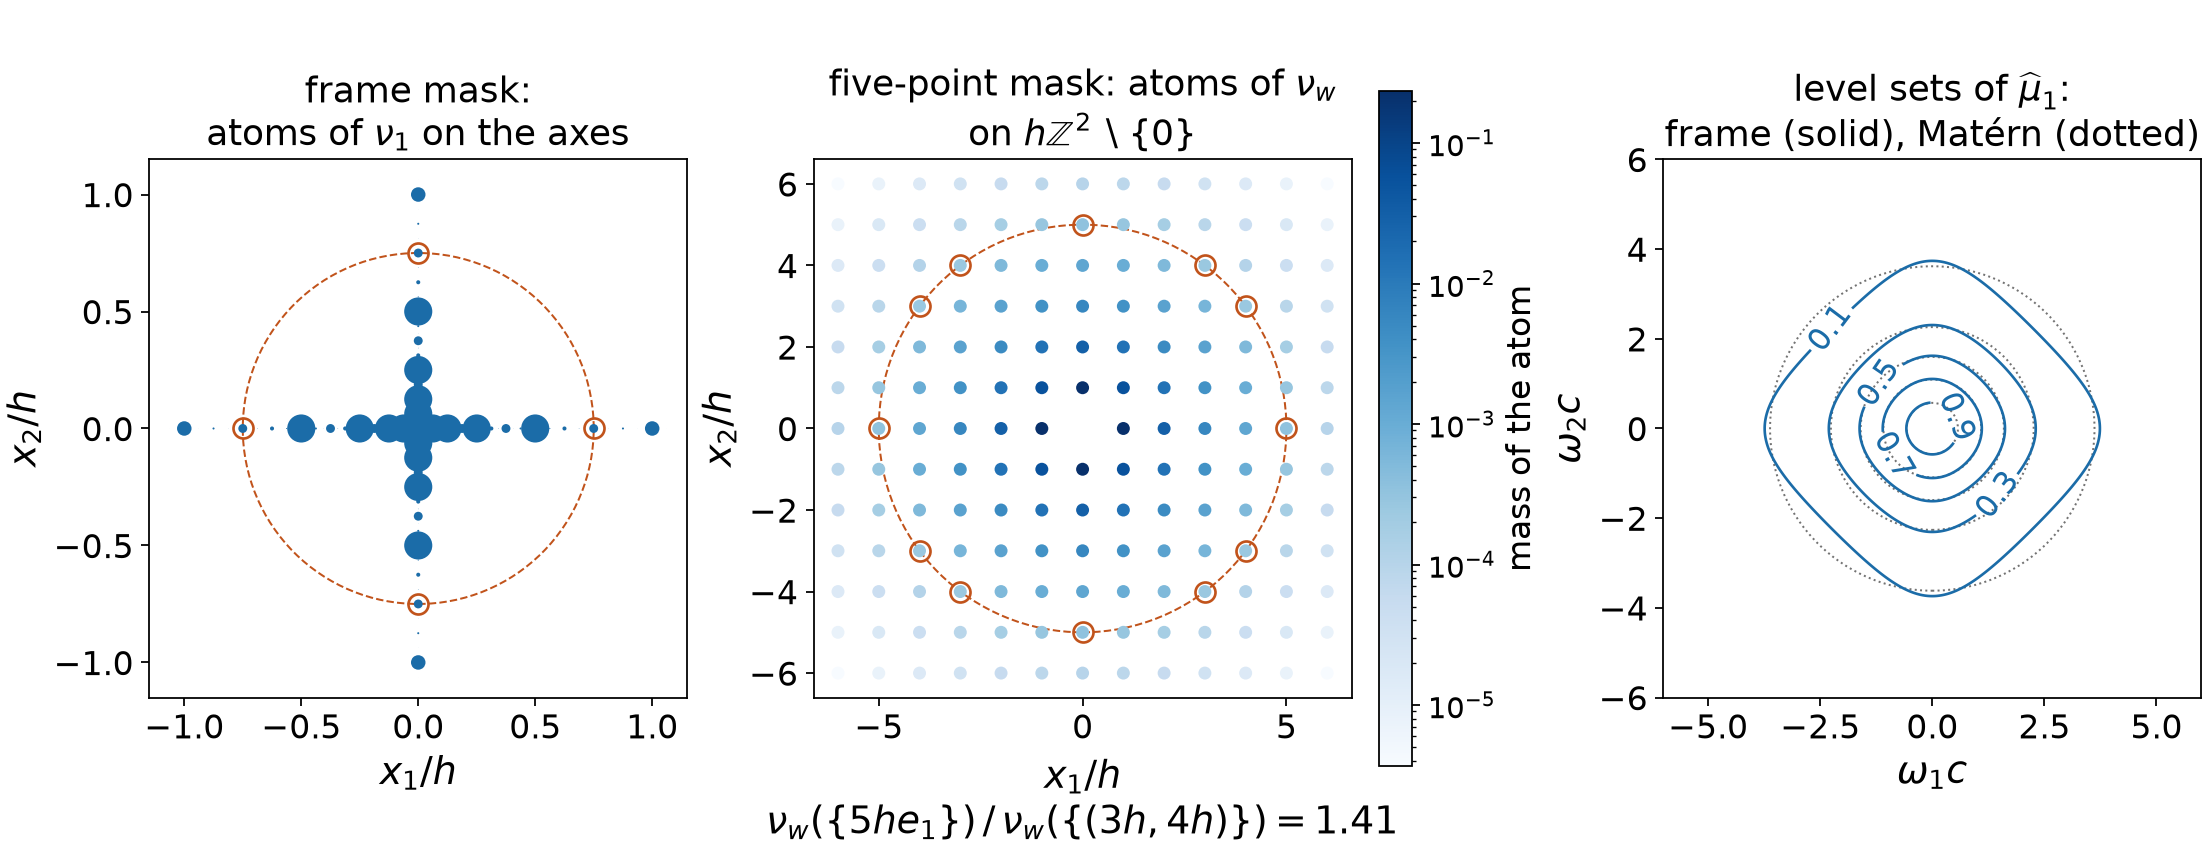
\includegraphics[width=\textwidth]{theory-frame.png}
\caption{Proposition~\ref{prop:grid-pyramid-not-isotropic}(3) on $h\ZZ^2$ with $q = 2$ and the
mask $(\lambda^{\mathrm L}_a)^{\otimes 2}$, $a = e^{-h/c}$ and $h/c = 1/2$: the sampled octave step
of the frame \Matern{} pyramid of range $c$. Left: the atoms of the \Levy{} measure $\nu_1$ of
(\ref{eq:frame-levy}) in the square $|x_i| \le 1.1h$, each of area proportional to its mass summed
over the terms $m \le 7$. The dashed circle of radius $3h/4$ meets the carrier of $\nu_1$ in its
four axis points. Middle, for comparison: the atoms of the \Levy{} measure $\nu_w$ of the five-point
resolvent mask $\kappa_t$ at $t = h$, so $p = 4/5$ in
Proposition~\ref{prop:resolvent-masks-exact}(4) and Proposition~\ref{prop:discrete-helmholtz}, on
$|x_i| \le 6h$, coloured by mass on a logarithmic scale. The series of
Proposition~\ref{prop:resolvent-masks-exact}(1) is summed over $k \le 143$, where $p^k/k$ falls
below $10^{-16}$, with each walk law computed without truncation, in double precision. Every lattice point but the origin is an atom. Of the points on the dashed circle
of radius $5h$, the twelve lattice points are atoms, with two different masses, in the ratio
$1.41$, and no other point is. Right: the level sets $0.1, 0.3, 0.5, 0.7, 0.9$ of $\widehat{\mu_1}$ (solid), against $\omega c$.
The dotted circles are the same level sets of $\exp(-F_q(|\omega|))$, the transform of the knot
kernel of the \Matern{} pyramid of Theorem~\ref{thm:matern-pyramid} with the same $q$ and $c$.
Along the diagonals the solid level sets $0.1$ to $0.7$ lie inside the circles. Both products
are cut at $m \le 59$. The solid level sets are traced by marching squares on a $601 \times 601$
mesh of $[-6, 6]^2$ in $\omega c$, and the dotted radii are read from $4000$ points of the radial
transform.}
\label{fig:theory-frame}
\end{figure}

The proof of clauses (1) and (2) reads of the dilation only that it is linear and invertible. So it
carries over to a dilation that also rotates the lattice, as in the quincunx filter banks
\cite[(2), p.~534]{kovacevic1992nonseparable} and the hexagonal pyramid
\cite[pp.~97, 99]{watson1989hexagonal}. The quincunx dilation $(x_1, x_2) \mapsto
(x_1 + x_2, x_1 - x_2)$ on $h\ZZ^2$ is $\sqrt2$ times a reflection. The proposition below assumes
neither that the dilation maps the lattice into itself nor that it is a multiple of an orthogonal
matrix, whose factor need not be the ratio $q$ of the scales.

% shared with blueprint prop:expanding-grid-pyramid-not-isotropic
\begin{proposition}[no exact grid pyramid with a matrix dilation is isotropic in $d \ge 2$]
\label{prop:expanding-grid-pyramid-not-isotropic}

Let $d \ge 2$, let $\Gamma \subset \RR^d$ be a full-rank lattice, let $w$ be a symmetric
probability law on $\Gamma$ with $w \ne \delta_0$, and let $M$ be an invertible real $d \times d$
matrix. Let $q > 1$, and let a family $(\mu_{s,t})_{0 \le s \le t}$ of probability laws on
$\RR^d$ have (a), (b) and (d) of Definition~\ref{def:exact-grid-pyramid} and, in place of (c),
\begin{enumerate}
\item[(c$_M$)] $\mu_{qs,qt} = M_*\mu_{s,t}$ for $0 \le s \le t$, where $M_*\mu$ is the image of
$\mu$ under $x \mapsto Mx$.
\end{enumerate}
Then no kernel $\mu_t$, $t > 0$, is rotation invariant. So no family with (a), (b), (c$_M$) and (d) makes the grid pyramid of $(w, M)$, the ladder $M^n_*w$ applied on the grids $M^n\Gamma$, isotropic in the sense of Definition~\ref{def:exact-grid-pyramid}.
\end{proposition}

\begin{proof}
Triplets are those of \ledger{A39}. They add under convolution, and the triplet of a law is unique.

\emph{The mask.} Every $\mu_{s,t}$ is infinitely divisible, by
Lemma~\ref{lem:steps-infinitely-divisible}, as in Proposition~\ref{prop:grid-pyramid-not-isotropic}(1).
The mask $w = \mu_{1,q}$ is carried by $\Gamma$, so by Lemma~\ref{lem:lattice-infinitely-divisible}
its triplet has Gaussian part $0$ and a finite \Levy{} measure $\nu_w$ carried by
$\Gamma \setminus \{0\}$, and $\nu_w \ne 0$ as $w \ne \delta_0$. A nonzero measure carried by a
countable set charges one of its points, so $\nu_w$ has an atom $b \ne 0$.

\emph{The steps.} By (c$_M$) at $(s/q, t/q)$, $\mu_{s,t} = M_*\mu_{s/q,t/q}$, and as $M$ is
invertible, $\mu_{s/q,t/q} = M^{-1}_*\mu_{s,t}$. By induction,
$\mu_{q^ks,q^kt} = M^k_*\mu_{s,t}$ for every integer $k$, and with (d),
$\mu_{q^{n-1},q^n} = M^{n-1}_*w$ for every integer $n$.

\emph{An atom of $\nu_t$.} Let $t > 0$, and choose an integer $n$ with $q^n \le t$. By (a),
\[
\mu_t = \mu_{q^{n-1}} * \mu_{q^{n-1},q^n} * \mu_{q^n,t} ,
\]
three infinitely divisible laws, so the \Levy{} measure $\nu_t$ of $\mu_t$ is the sum of theirs. By
\ledger{A42} with $U = M^{n-1}$, the \Levy{} measure of $\mu_{q^{n-1},q^n} = M^{n-1}_*w$ is
$M^{n-1}_*\nu_w$, as $M^{n-1}$ maps only $0$ to $0$. So $\nu_t \ge M^{n-1}_*\nu_w$, and the point
$x := M^{n-1}b \ne 0$ has $\nu_t(\{x\}) \ge \nu_w(\{b\}) > 0$.

\emph{No isotropy.} Suppose $\mu_t$ is invariant under $\mathrm{SO}(d)$. For
$R \in \mathrm{SO}(d)$, \ledger{A42} with $U = R$ gives the \Levy{} measure $R_*\nu_t$ to
$D_R\mu_t = \mu_t$, so $R_*\nu_t = \nu_t$ by uniqueness, and $\nu_t(\{Rx\}) = \nu_t(\{x\})$. As
$d \ge 2$, every point $y$ of the sphere $\{|y| = |x|\}$ is $Rx$ for some $R \in \mathrm{SO}(d)$, and
the sphere is infinite, both as in the proof of Proposition~\ref{prop:grid-pyramid-not-isotropic}(2).
So for every $N$ the sphere holds $N$ distinct points of mass $\nu_t(\{x\}) > 0$ each, and
$\nu_t(\{|y| \ge |x|\}) \ge N\nu_t(\{x\})$. But a \Levy{} measure is finite off every
neighbourhood of $0$, and $|x| > 0$. This contradiction proves the first sentence; the second is the
first, read through the definition of isotropy.

The cited facts are
\ledger{A41}, \ledger{A39} and \ledger{A42}, with \ledger{A48} through
Lemma~\ref{lem:lattice-infinitely-divisible}.
\end{proof}

\emph{On the line.} In $d = 1$ the exact grid pyramids are those that are exact in the sense of
Definition~\ref{def:grid-pyramid-line}, a definition on operators
(Proposition~\ref{prop:line-and-arrays}(1)). There Proposition~\ref{prop:grid-pyramid-not-isotropic}(2)
is empty, since $\Orth(1) = \{\pm 1\}$, and clause (1) is the product formula of
Proposition~\ref{prop:grid-pyramids-infinitely-divisible}(2) on $\Gamma = h\ZZ$.

For an integer ratio the kernels of an exact grid pyramid have no density at all, in every
dimension. The mask is carried by the grid, so its transform is $1$ on the dual grid. The knot
relation then keeps the transform of the knot kernel equal to one value along a sequence of
frequencies that tends to infinity. Clause (3) of the next proposition strengthens this to
singularity.

% shared with blueprint prop:grid-pyramid-singular-kernels
\begin{proposition}[the kernels of an exact grid pyramid are singular]
\label{prop:grid-pyramid-singular-kernels}

Let $q \ge 2$ be an integer and $h > 0$, and let $(w, q)$ be an exact grid pyramid on $h\ZZ^d$,
carried by the family $(\mu_{s,t})$.
\begin{enumerate}
\item \emph{(One value along a ray.)} For every coordinate vector $e_i$,
\[
  \widehat{\mu_1}\bigl(2\pi q^ke_i/h\bigr) = \widehat{\mu_1}\bigl(2\pi e_i/h\bigr) \ne 0,
  \qquad k \ge 0 .
\]
\item \emph{(No density.)} No kernel $\mu_t$, $t > 0$, is absolutely continuous with respect to
Lebesgue measure.
\item \emph{(Singular.)} Every kernel $\mu_t$, $t > 0$, is singular with respect to Lebesgue
measure: it is carried by a Lebesgue-null set.
\end{enumerate}
\end{proposition}

\begin{proof}
Write $\xi := 2\pi e_i/h$ and $G := h\ZZ[1/q]^d$, which is
$\bigcup_{k \ge 0}q^{-k}h\ZZ^d$ (Proposition~\ref{prop:grid-pyramid-not-isotropic}(1)).

(1) By (a), (c) and (d), $D_q\mu_1 = \mu_{0,q} = \mu_1 * w$, so
$\widehat{\mu_1}(q\omega) = \widehat{w}(\omega)\,\widehat{\mu_1}(\omega)$, as in the proof of
Lemma~\ref{lem:knot-data}. For $k \ge 0$ and $n \in \ZZ^d$,
$\langle q^k\xi, hn\rangle = 2\pi q^kn_i$ is an integer multiple of $2\pi$, $q$ being an integer.
So $e^{i\langle q^k\xi, x\rangle} = 1$ at every point $x$ of $h\ZZ^d$, which carries $w$, and
$\widehat w(q^k\xi) = 1$. Hence $\widehat{\mu_1}(q^{k+1}\xi) = \widehat{\mu_1}(q^k\xi)$, and by
induction $\widehat{\mu_1}(q^k\xi) = \widehat{\mu_1}(\xi)$ for every $k \ge 0$. The law
$\mu_1 = \mu_{0,1}$ is infinitely divisible, by Lemma~\ref{lem:steps-infinitely-divisible}, so its
transform has no zero (\ledger{A40}).

(2) Let $t > 0$, and choose an integer $n \ge 0$ with $t \le q^n$. By (a),
$\mu_{q^n} = \mu_t * \mu_{t,q^n}$, so $\widehat{\mu_{q^n}} = \widehat{\mu_{t,q^n}}\,\widehat{\mu_t}$,
and as the transform of a probability law has modulus at most $1$,
$|\widehat{\mu_t}(\omega)| \ge |\widehat{\mu_{q^n}}(\omega)|$ for every $\omega$. By (c),
$\mu_{q^n} = D_{q^n}\mu_1$, so at $\omega_k := q^k\xi$ (1) gives
$\widehat{\mu_{q^n}}(\omega_k) = \widehat{\mu_1}(q^{n+k}\xi) = \widehat{\mu_1}(\xi)$. So
$|\widehat{\mu_t}(\omega_k)| \ge |\widehat{\mu_1}(\xi)| > 0$ for every $k$, while
$|\omega_k| = 2\pi q^k/h \to \infty$. If $\mu_t$ had a density, its transform would tend to $0$ at
infinity, by the Riemann--Lebesgue lemma. So $\mu_t$ is not absolutely continuous.

(3) \emph{A random series.} Let $X_1, X_2, \dots$ be independent random vectors, $X_m$ with law
$D_{q^{-m}}w$, and $T_M := X_1 + \dots + X_M$, $T_0 := 0$, whose law is
$\rho_M := D_{q^{-1}}w * \dots * D_{q^{-M}}w$. By (\ref{eq:knot-product}), $\rho_M \to \mu_1$
weakly. A weakly convergent sequence of probability laws on $\RR^d$ is tight: for $\eta > 0$ there
is $R$ with $\rho_j(\{|x| > R\}) < \eta$ for every $j$. For $M < M'$ the difference
$T_{M'} - T_M = X_{M+1} + \dots + X_{M'}$ has the law $D_{q^{-M}}\rho_{M'-M}$, so for
$\varepsilon > 0$,
\[
  P\bigl(|T_{M'} - T_M| > \varepsilon\bigr) = \rho_{M'-M}\bigl(\{|x| > q^M\varepsilon\}\bigr) < \eta
  \qquad\text{once } q^M\varepsilon \ge R .
\]
So $(T_M)$ is a Cauchy sequence in probability. It converges in probability to a random vector
$S$, and almost surely along a subsequence, and the law of $S$ is the weak limit of the $\rho_M$,
which is $\mu_1$.

\emph{A zero-one law.} Each $X_m$ takes its values in $q^{-m}h\ZZ^d \subseteq G$. The set $G$ is a
group, the union of the increasing groups $q^{-k}h\ZZ^d$ (increasing as $q$ is an integer), so
$T_M \in G$ for every $M$. Let $A \subseteq \RR^d$ be a Borel set with $A + g = A$ for every
$g \in G$, and $E := \{S \in A\}$. Then $E = \{S - T_M \in A\}$ for every $M$. The vector
$S - T_M$ is the limit in probability of $T_{M'} - T_M$ as $M' \to \infty$, so it agrees almost
surely with the limit along a subsequence, a function of $X_{M+1}, X_{M+2}, \dots$. So $E$ agrees
almost surely with an event $E_M$ of $\mathcal{F}_M := \sigma(X_{M+1}, X_{M+2}, \dots)$, for every
$M \ge 0$. The event $E_M$ is independent of $\sigma(X_1, \dots, X_M)$, and so is $E$, which
differs from it by a null set. The union of the $\sigma(X_1, \dots, X_M)$, $M \ge 1$, is a
$\pi$-system that generates $\mathcal{F}_0$, so by the $\pi$--$\lambda$ theorem $E$ is independent
of $\mathcal{F}_0$, which contains $E_0$. Then $P(E) = P(E \cap E_0) = P(E)\,P(E_0) = P(E)^2$, and
$\mu_1(A) = P(E)$ is $0$ or $1$. This is Kolmogorov's zero-one argument as Jessen and Wintner use
it for their law of pure types [\sscite{jessen1935distribution}, Thm.~35, p.~86],
[\sscite{sato1999levy}, Prop.~27.18, p.~182].

\emph{The knot kernel is singular.} By (2), $\mu_1$ is not absolutely continuous, so some Borel set
$N$ of Lebesgue measure $0$ has $\mu_1(N) > 0$. The set $A := N + G = \bigcup_{g \in G}(N + g)$ is a
countable union of null Borel sets, so it is a null Borel set, and $A + g = A$ for $g \in G$. As
$\mu_1(A) \ge \mu_1(N) > 0$, the zero-one law gives $\mu_1(A) = 1$: $\mu_1$ is carried by the null
set $A$.

\emph{Every kernel.} Let $t > 0$, and choose $n \in \ZZ$ with $q^n \le t < q^{n+1}$. By (a),
$\mu_t = \mu_{q^n} * \mu_{q^n,t}$, and $\mu_{q^n} = D_{q^n}\mu_1$ is carried by the null set
$q^nA$. The step $\mu_{q^n,t}$ is carried by a countable set. Indeed, by (a), (c) and (d),
$D_{q^n}w = \mu_{q^n,q^{n+1}} = \mu_{q^n,t} * \mu_{t,q^{n+1}}$, three infinitely divisible laws
(Lemma~\ref{lem:steps-infinitely-divisible}), whose triplets of \ledger{A39} add. By
Proposition~\ref{prop:grid-pyramid-not-isotropic}(1) the mask has the data $(0, \nu_w)$ with
$\nu_w$ finite and carried by $h\ZZ^d \setminus \{0\}$, so the symmetric law $D_{q^n}w$ has the
triplet $(0, D_{q^n}\nu_w, 0)$. Two positive semidefinite Gaussian parts with sum $0$ vanish, so
$\mu_{q^n,t}$ has a triplet $(0, \nu', \gamma')$ with $\nu' \le D_{q^n}\nu_w$, a finite measure
carried by $q^nh\ZZ^d$. Its transform is therefore
$\exp\bigl(i\langle b, \omega\rangle + \int(e^{i\langle\omega, x\rangle} - 1)\,\nu'(dx)\bigr)$ with
$b := \gamma' - \int_{\{|x| \le 1\}}x\,\nu'(dx)$, the transform of
$\delta_b * e^{-\nu'(\RR^d)}\sum_{k \ge 0}\nu'^{*k}/k!$. So $\mu_{q^n,t}$ is this law, carried by
the countable set $C := b + q^nh\ZZ^d$. The set $q^nA + C$ is a countable union of translates of
$q^nA$, so it is null, and
\[
  \mu_t(q^nA + C) = \int\mu_{q^n}(q^nA + C - y)\,\mu_{q^n,t}(dy) = 1,
\]
since $q^nA + C - y \supseteq q^nA$ for $y \in C$. So $\mu_t$ is singular.

Clauses (1) and (2) are machine-checked, and their cited facts are \ledger{A40} and \ledger{A41};
clause (3) is proved here in print only, with \ledger{A39} and the entries of
Proposition~\ref{prop:grid-pyramid-not-isotropic}(1).
\end{proof}

The proof of (1) and (2) reads of the grid only a point $\xi \ne 0$ of its dual, with
$\langle\xi, \gamma\rangle \in 2\pi\ZZ$ for every $\gamma$ of the lattice. Every full-rank lattice
has one, so (1) and (2) hold on every full-rank lattice, with $\xi$ in place of $2\pi e_i/h$. The
pyramid principle, which reads continuous densities, therefore never applies to a family that
carries an exact grid pyramid of integer ratio.

The frame pyramid on the grid is exact, and by clause (2) it is not isotropic in $d \ge 2$.
Section~\ref{ch:matern} tests a pyramid in a second way, by the implicit-Euler principle of
Definition~\ref{def:implicit-euler-principle}. At a local maximum of the output, the output does
not exceed the input, and at a local minimum it is not below it. On the continuum this test rejects
the octave step of the frame pyramid, while each of its axis passes has the principle
(Theorem~\ref{thm:selection-stratum-two}(4)). On the grid a local maximum is read on a finite
symmetric neighbourhood $\mathcal{N}$ of lattice points. The next proposition shows that the grid
gives the same verdict, in every dimension $d \ge 2$.

% shared with blueprint prop:grid-frame-step-not-selected
\begin{proposition}[the frame step on the grid is not selected]
\label{prop:grid-frame-step-not-selected}

Let $d \ge 2$, $h > 0$ and $0 < a < 1$, and let $w := (\lambda^{\mathrm L}_a)^{\otimes d}$ be the
frame mask on $h\ZZ^d$ of Proposition~\ref{prop:grid-pyramid-not-isotropic}(3), the octave step of
the frame \Matern{} pyramid on the grid. Let $\mathcal{N}$ range over the finite symmetric sets of
nonzero points of $h\ZZ^d$, and read the principle on $\mathcal{N}$ as in
Definition~\ref{def:implicit-euler-principle}.
\begin{enumerate}
\item For every such $\mathcal{N}$, the frame mask $w$ does not have the principle on $\mathcal{N}$.
\item For each $i$, the axis pass along $e_i$, the law $\lambda^{\mathrm L}_a$ carried by the axis
$h\ZZ e_i$, has the principle on $\mathcal{N}$ for every such $\mathcal{N}$ that contains $\pm he_i$.
\end{enumerate}
\end{proposition}

\begin{proof}
We read kernels on $h\ZZ^d$ in their indices $n \in \ZZ^d$, so that $he_i$ is the index $e_i$ and
$h$ plays no further role; $\lambda := \lambda^{\mathrm L}_a$ is a kernel on $\ZZ$. Put
$\varsigma := a/(1-a)^2 > 0$.

\emph{The inverse on the line.} The values of $\lambda$ satisfy the three-point recursion
\[
(1 + 2\varsigma)\lambda(m) - \varsigma\bigl(\lambda(m+1) + \lambda(m-1)\bigr) = \delta_0(m),
\qquad m \in \ZZ .
\]
Indeed, let $c := \tfrac{1-a}{1+a}$, and note $\varsigma(1-a)^2 = a$. For $m \ne 0$ the left side
is $c\,a^{|m|-1}\bigl((1 + 2\varsigma)a - \varsigma(1 + a^2)\bigr) = c\,a^{|m|-1}\bigl(a -
\varsigma(1-a)^2\bigr) = 0$. For $m = 0$ it is $c\,(1 + 2\varsigma(1-a)) = c\,(1 + 2a/(1-a)) = 1$.
So the kernel $m_1 := (1 + 2\varsigma)\delta_0 - \varsigma(\delta_1 + \delta_{-1})$, carried by
$\{-1, 0, 1\}$, has $m_1 * \lambda = \delta_0$.

\emph{The inverse of the frame mask.} Let $M := m_1^{\otimes d}$, $M(n) := \prod_jm_1(n_j)$, a
kernel carried by the box $B := \{-1, 0, 1\}^d$. For a kernel $g$ on $\ZZ$ and $n \in \ZZ^d$, the
convolution $(M * g^{\otimes d})(n)$ is a finite sum over $B$, and expanding a product of $d$ finite
sums gives
\[
(M * g^{\otimes d})(n) = \sum_{y \in B}\prod_jm_1(y_j)\,g(n_j - y_j)
= \prod_j\,\sum_{y_j \in \{-1, 0, 1\}}m_1(y_j)\,g(n_j - y_j) .
\]
At $g = \lambda$ each factor is $\delta_0(n_j)$ by the recursion, so $M * w = \delta_0$. The mask
$w$ is summable: a finite set of indices lies in the box of its coordinates, over which the sum of
$w$ is a product of $d$ finite sums of $\lambda$, each at most $1$. Convolution of two summable
kernels is associative against a bounded function, since the double sum converges absolutely,
by the product of the two masses and the bound.

(1) Let $u := -1$ on the set $D$ of the four indices $\pm e_1 \pm e_2$ and $u := 0$ elsewhere, and
let $f := M * u$, bounded since $M$ is finitely supported and $u$ is bounded. Then
$w * f = (w * M) * u = u$, as $w * M = M * w = \delta_0$, convolution of summable kernels being
commutative. Since $u \le 0 = u(0)$, the origin is a maximum of $u$ over the whole
grid, so it is an $\mathcal{N}$-maximum for every $\mathcal{N}$. Next,
$f(0) = \sum_yM(y)\,u(-y)$. A term is nonzero only if $-y \in D$, that is $y \in D$, and there
$y_1, y_2 \in \{\pm1\}$ and $y_j = 0$ for $j \ge 3$, so
\[
M(y) = m_1(\pm1)\,m_1(\pm1)\prod_{j \ge 3}m_1(0) = \varsigma^2(1 + 2\varsigma)^{d-2} > 0 .
\]
So every term of $f(0)$ is $\le 0$, the four nonzero ones are $-\varsigma^2(1 + 2\varsigma)^{d-2}$,
and
\[
f(0) = -4\varsigma^2(1 + 2\varsigma)^{d-2} < 0 = u(0) .
\]
The principle would require $u(0) \le f(0)$ at an $\mathcal{N}$-maximum, so it fails. At $d = 2$,
$f(0) = -4\varsigma^2$.

(2) Let $\kappa$ be the law $\lambda$ carried by the axis $\ZZ e_i$, and
$m^{(i)} := (1 + 2\varsigma)\delta_0 - \varsigma(\delta_{e_i} + \delta_{-e_i})$. Then
$(m^{(i)} * \kappa)(n) = (1 + 2\varsigma)\kappa(n) - \varsigma\bigl(\kappa(n + e_i) +
\kappa(n - e_i)\bigr)$. If $n$ lies on the axis, so do $n \pm e_i$, and this is the recursion at
$n_i$, equal to $\delta_0(n_i) = \delta_0(n)$. Otherwise $n$ has a nonzero coordinate $n_j$,
$j \ne i$, which $n \pm e_i$ share, so the three values of $\kappa$ vanish, and so does
$\delta_0(n)$. So $m^{(i)} * \kappa = \delta_0$, and $\kappa$ is summable, its values being those
of $\lambda$. For a bounded $f$ and $u := \kappa * f$, associativity gives
$f = (m^{(i)} * \kappa) * f = m^{(i)} * u$, that is
\[
f(x) = u(x) + \varsigma\bigl(2u(x) - u(x + e_i) - u(x - e_i)\bigr) .
\]
At an $\mathcal{N}$-maximum $x$ of $u$ with $\pm e_i \in \mathcal{N}$ the bracket is nonnegative,
so $u(x) \le f(x)$. At an $\mathcal{N}$-minimum it is nonpositive, so $f(x) \le u(x)$.

Every step is machine-checked, with no cited fact.
\end{proof}

The proof reads the failure off the inverse of the mask. The inverse of an axis pass has
nonpositive weights off the origin. The inverse $M$ of the frame mask is the tensor power of those,
and it charges the diagonal neighbours $\pm he_1 \pm he_2$ with the positive weight
$\varsigma^2(1 + 2\varsigma)^{d-2}$. In the counterexample the origin is a maximum over the whole
grid, so the failure does not depend on the neighbourhood.

The signs of the inverse are what the principle reads, as follows. With $u := w * f$ and
$M * w = \delta_0$, the input is $f = M * u$. The weights of $M$ sum to $1$, so
$f(x) - u(x) = \sum_{y \ne 0}M(y)\bigl(u(x - y) - u(x)\bigr)$. At an $\mathcal{N}$-maximum $x$ of
$u$, every bracket with $y \in \mathcal{N}$ is at most $0$. So an inverse with nonpositive weights
off the origin, carried by $\mathcal{N} \cup \{0\}$, gives $u(x) \le f(x)$. A positive weight off
the origin can break it.

\subsection{Which masks are exact, and what the algorithm computes}
\label{sec:price-masks}

Section~\ref{sec:price-obstruction} showed what an exact pyramid on a lattice gives up. This
subsection turns to what a designer can still choose. Which masks give an exact pyramid, and what
does the pyramid algorithm compute with them? Proposition~\ref{prop:grid-pyramid-not-isotropic}(1)
gives a necessary condition: the mask is infinitely divisible. With a logarithmic moment the
condition is also sufficient, in every dimension. For laws the sufficiency is the theorem of
Maejima and Ueda [\sscite{maejima2009stochastic}, Thm.~3.3, p.~353]. Necessity follows from
continuity in scale (Lemma~\ref{lem:steps-infinitely-divisible}). The criterion does not involve
$q$, so a mask that is exact for one ratio is exact for every ratio. It can be tested on the
weights. By Proposition~\ref{prop:exact-masks}(1) an infinitely divisible mask on a lattice is
compound Poisson, so its transform is positive, and the logarithm of the transform has the absolutely
summable Fourier coefficients $\nu_w(\{x\}) \ge 0$ at the points $x \ne 0$. Conversely, a symmetric
mask whose transform is positive, with a logarithm of that kind, is the compound Poisson law of
those coefficients, and so it is infinitely divisible.
\begin{itemize}
\item Proposition~\ref{prop:exact-masks} gives the criterion. It also shows that the ladder fixes
the knot kernels but not the family between them.
\item Proposition~\ref{prop:resolvent-masks-exact} shows that the resolvent masks of a random walk
whose step has a logarithmic moment meet the criterion. A comparison with the frame mask under the
implicit-Euler principle follows it.
\item Definition~\ref{def:level-records} to Proposition~\ref{prop:binomial-records} follow an
input through the levels of the computed pyramid. In $d \ge 2$ and for an integer $q \ge 2$, one
level can create local maxima, for two exact masks and for the binomial mask.
\item Proposition~\ref{prop:line-and-arrays} says what the algorithm returns. It also shows that on
the line the two definitions of an exact grid pyramid agree.
\item Proposition~\ref{prop:binomial-knot-relation} shows why the definition requires continuity in
scale.
\end{itemize}

% shared with blueprint prop:exact-masks
\begin{proposition}[which laws have an exact ladder]
\label{prop:exact-masks}

Let $w \ne \delta_0$ be a symmetric probability law on $\RR^d$ and $q > 1$.
\begin{enumerate}
\item \emph{(Criterion.)} The following are equivalent.
\begin{enumerate}
\item[(a)] The ladder of $(w, q)$ is exact.
\item[(b)] $w$ is infinitely divisible and $\int\log_+|x|\,\nu_w(dx) < \infty$.
\item[(c)] $w$ is infinitely divisible and $\int\log_+|x|\,w(dx) < \infty$.
\end{enumerate}
If $w$ is carried by a full-rank lattice $\Gamma$, an infinitely divisible $w$ is the compound
Poisson law with a finite symmetric \Levy{} measure $\nu_w$ carried by $\Gamma \setminus \{0\}$, and
its support is unbounded.
\item \emph{(Ladder and family.)} Let $w$ be carried by a full-rank lattice $\Gamma$. If (a)--(c)
hold, the knot
kernel $\mu_1$ is that of
(\ref{eq:knot-product}), with no Gaussian part and \Levy{} measure $\nu^* := \sum_{m \ge 1}
D_{q^{-m}}\nu_w$. The families carrying the ladder are not unique. One of them is the
\emph{uniform coupling}, with \Levy{} measures $\nu_t := \nu^* + (\log_qt)\,\nu_w$ for
$t \in [1, q]$, $\nu_{q^nt} := D_{q^n}\nu_t$, and no Gaussian part.
\end{enumerate}
\end{proposition}

\begin{proof}
\emph{Data.} A symmetric infinitely divisible law has unique \Levy{} data $(A, \nu)$, so a unique
\Levy{} measure, and the triplet $(2A, \nu, 0)$, by Lemma~\ref{lem:symmetric-levy-khintchine}.
Data add under convolution, the exponents adding, and $D_c\mu$ has the data $(c^2A, D_c\nu)$ by the
substitution $y = cx$.

(1) \emph{The last sentence.} Let $w$ be carried by $\Gamma$ and infinitely divisible, with data
$(A_w, \nu_w)$. By
Lemma~\ref{lem:lattice-infinitely-divisible}, $A_w = 0$ and $\nu_w$ is finite and carried by
$\Gamma \setminus \{0\}$. So $\widehat w = e^{-\psi_w}$ with $\psi_w(\omega) := \int(1 -
\cos\langle\omega, x\rangle)\,\nu_w(dx)$, the transform of the compound Poisson law
$e^{-\nu_w(\RR^d)}\sum_{k \ge 0}\nu_w^{*k}/k!$ of the symmetric measure $\nu_w$, and by the uniqueness
of the transform $w$ is that law. It is not a point mass, a symmetric $\delta_x$ being $\delta_0$.
By Proposition~\ref{prop:no-bounded-step}, a law of bounded support that is not a point mass is not
infinitely divisible, so the support of $w$ is unbounded: $w(\{|x| > R\}) > 0$ for every $R$.

\emph{(a) implies (b).} Let $(\mu_{s,t})$ carry the ladder. Every $\mu_{s,t}$ is infinitely
divisible, by Lemma~\ref{lem:steps-infinitely-divisible}, which applies since $d \ge 1$, $w$ being
a law other than $\delta_0$. Its (I1) is condition (a) of Definition~\ref{def:exact-grid-pyramid},
convolution being commutative, and its (I2) follows from the weak continuity (b) there, as
$x \mapsto e^{i\langle\omega, x\rangle}$ is bounded and continuous. So $w = \mu_{1,q}$ is
infinitely divisible, and it has data $(A_w, \nu_w)$. By Lemma~\ref{lem:knot-data}, $\mu_1$ has the
data $(A_w/(q^2 - 1), \nu^*)$, with $\nu^* := \sum_{m \ge 1}D_{q^{-m}}\nu_w$. So $\nu^*$ is a
\Levy{} measure, and by Tonelli
\[
\int\min\bigl(1, |x|^2\bigr)\,\nu^*(dx) = \int\Bigl[\sum_{m \ge 1}\min\bigl(1,
q^{-2m}|v|^2\bigr)\Bigr]\,\nu_w(dv) < \infty .
\]
For $|v| > 1$ the $\lfloor\log_q|v|\rfloor$ terms of the bracket with $q^m \le |v|$ equal $1$, so
the bracket is at least $\log_q|v| - 1$. Hence
$\log_+|v| \le \log q\,\bigl(\text{bracket} + \mathbf 1_{\{|v| > 1\}}\bigr)$ for every $v$, and
$\nu_w(\{|v| > 1\}) < \infty$ gives $\int\log_+|x|\,\nu_w(dx) < \infty$. This is
Proposition~\ref{prop:ladder-knot-kernel}(1)'s last sentence, for a family assumed only to carry
the ladder.

\emph{(b) implies (a).} The mask $w$ is a symmetric infinitely divisible law other than $\delta_0$
with $\int\log_+|x|\,\nu_w(dx) < \infty$. By Proposition~\ref{prop:ladder-knot-kernel}(2) some
symmetric $q$-covariant family with $S_qt = qt$ has $\mu_{1,q} = w$. Its cascade (I1) is (a) of
Definition~\ref{def:exact-grid-pyramid}, convolution being commutative; the continuity (I2) of its
transforms gives the weak continuity (b) by \Levy's continuity theorem; its covariance at $q$ with
$S_qt = qt$ is (c); and $\mu_{1,q} = w$ is (d). So the ladder is exact.

\emph{(b) is equivalent to (c).} This is the equivalence of the two logarithmic moments in
Proposition~\ref{prop:ladder-knot-kernel}(2), whose proof reads \ledger{A49} with
$g(x) = \log(|x| \vee e)$.

(2) Let the conditions hold, and let $(A_w, \nu_w)$ be the data of $w$, so that $A_w = 0$ by (1).
Let $(\mu_{s,t})$ carry the ladder. As $w$ is carried by $\Gamma$, the ladder is an exact grid
pyramid on the lattice $\Gamma$, so
by Proposition~\ref{prop:grid-pyramid-not-isotropic}(1) the knot kernel is (\ref{eq:knot-product}),
with no Gaussian part and the \Levy{} measure $\nu_{q^0} = \sum_{m \ge 1}D_{q^{-m}}\nu_w = \nu^*$.

Families carrying the ladder are built by Lemma~\ref{lem:synthesis} from data on one octave. For a
weight $\ell$, continuous and strictly increasing on $[1, q]$ with $\ell(1) = 0$ and $\ell(q) = 1$,
take the data $(0, \nu_u)$, $\nu_u := \nu^* + \ell(u)\,\nu_w$, $u \in [1, q]$. Their exponents
$\Psi^*(\xi) + \ell(u)\psi_w(\xi)$, with $\Psi^*$ the exponent of $(0, \nu^*)$, are continuous in $u$;
they increase strictly, as $\psi_w \not\equiv 0$ for $w \ne \delta_0$; and they glue, as
$D_q\nu^* = \nu_w + \nu^*$. The lemma extends them to every $t = q^nu$, $u \in [1, q)$, by
$\nu_t := D_{q^n}\nu_u$, and gives laws $\mu_{s,t}$ with the transforms $e^{-(\Psi_t - \Psi_s)}$,
$\Psi_t$ the exponent of $(0, \nu_t)$ and $\Psi_0 = 0$. They form a symmetric $q$-covariant family
with $S_qt = qt$, and $\mu_{1,q}$ has the transform $e^{-(\Psi_q - \Psi_1)} = e^{-\psi_w}$, so it is
$w$, and the family meets (a)--(d) as in (b) implies (a): it carries the ladder.

\emph{Not unique.} The weights $\log_qu$ and $(\log_qu)^2$ give two such families. At
$t = q^{1/2}$ their laws $\mu_{1,t}$ have the exponents $\tfrac12\psi_w$ and $\tfrac14\psi_w$, which
differ where $\psi_w \ne 0$.

\emph{The uniform coupling} is the family of the weight $\log_q$. Its kernel $\mu_t = \mu_{0,t}$,
$t > 0$, has the transform $e^{-\Psi_t}$, so it has the data $(0, \nu_t)$: at $t = q^nu$ with
$n = \lfloor\log_qt\rfloor$ and $u = q^{-n}t \in [1, q)$, the \Levy{} measure
$D_{q^n}\bigl(\nu^* + (\log_qu)\,\nu_w\bigr)$, the measure $\nu_t$ of the statement.

Every step is machine-checked, and the cited facts are \ledger{A41}, \ledger{A39} and those of the
statements used.
\end{proof}

\emph{On the line.} Proposition~\ref{prop:exact-masks} is
Proposition~\ref{prop:grid-pyramids-infinitely-divisible}(1)--(2), with the same logarithmic
moment.

For a pyramid as it is built, clause (1) means that an exact mask on a lattice has unbounded
support. So no finite mask is exact, and truncating an exact mask makes it inexact. Clause (2)
means that the ladder fixes the knot kernels but not the laws between the knots. Two families can
carry the same ladder and differ inside an octave.

An exact mask must then be applied without truncation. On the infinite grid the resolvents of
discrete Laplacians can be. Applied to a bounded array $f$ on $h\ZZ^d$, the $(2d+1)$-point
resolvent $\kappa_t$ gives $v := \kappa_t * f$, a bounded solution of $(1 - t^2\Delta_h)v = f$,
with no truncation of $\kappa_t$. It is the only bounded one: the difference of two, added to
$\kappa_t$, would be a second bounded solution of $(1 - t^2\Delta_h)\kappa = \delta_0$
(Proposition~\ref{prop:discrete-helmholtz}(1)). Finite arrays,
with their boundaries, are left to the further work named in Section~\ref{sec:discrete-helmholtz}.
The next proposition shows that these masks are exact. Each is the law of a lattice random walk stopped at an independent
geometric time, and its \Levy{} measure is a series in the convolution powers of the step.

% shared with blueprint prop:resolvent-masks-exact
\begin{proposition}[the resolvent masks are exact]
\label{prop:resolvent-masks-exact}

Let $\sigma \ne \delta_0$ be a symmetric probability law on $\Gamma$, let $0 < p < 1$, and let
\begin{equation}\label{eq:resolvent-mask}
w := (1 - p)\sum_{k \ge 0}p^k\sigma^{*k}, \qquad \widehat{w} = \frac{1 - p}{1 - p\,\widehat{\sigma}} .
\end{equation}
\begin{enumerate}
\item $w$ is infinitely divisible. It is the compound Poisson law whose \Levy{} measure $\nu_w$ is
the restriction of $\sum_{k \ge 1}\tfrac{p^k}{k}\sigma^{*k}$ to $\Gamma \setminus \{0\}$, of total
mass at most $\log\frac{1}{1-p}$.
\item Let $\int\log_+|x|\,\sigma(dx) < \infty$, as when $\sigma$ has finite support. For every
$q > 1$ and every integer $\gamma \ge 1$ the grid pyramid of $(w^{*\gamma}, q)$ is exact, with the
knot kernel
$\widehat{\mu_1} = \prod_{m \ge 1}\widehat{w}(q^{-m}\,\cdot)^\gamma$.
\item If $d \ge 2$ and $\operatorname{supp}\sigma$ spans $\RR^d$, then for every $q > 1$ and every
integer $\gamma \ge 1$ no kernel $\mu_t$, $t > 0$, of a family carrying the ladder of
$(w^{*\gamma}, q)$ is rotation invariant. At every knot the symmetry group of the kernel is
finite, and it contains every $R \in \Orth(d)$ with $R_*\sigma = \sigma$.
\item \emph{(Instances.)} Let $\Gamma = h\ZZ^d$, and let $t > 0$, in this clause the range of a
resolvent, not a scale of the pyramid. The $(2d+1)$-point resolvent $\kappa_t$ of
Proposition~\ref{prop:discrete-helmholtz} is (\ref{eq:resolvent-mask}) with $\sigma$ the simple
random walk step and $p = 2dt^2/(h^2 + 2dt^2)$, and then $\nu_w$ charges every nonzero point
of $h\ZZ^d$. On $h\ZZ^2$ the nine-point resolvent $\kappa^9_t$ of
Proposition~\ref{prop:nine-point-family} is (\ref{eq:resolvent-mask}) with its step $\sigma_9$ and
$p = 10t^2/(3h^2 + 10t^2)$. More generally, a mask with
$1/\widehat{w}(\omega) = 1 + \sum_{y \in \mathcal{N}}c_y\bigl(1 - \cos\langle\omega, y\rangle\bigr)$,
for a finite symmetric $\mathcal{N} \subset \Gamma \setminus \{0\}$ and $c_y = c_{-y} \ge 0$ not
all $0$, is (\ref{eq:resolvent-mask}) with $C := \sum_yc_y$, $p := C/(1 + C)$ and
$\sigma := (2C)^{-1}\sum_yc_y(\delta_y + \delta_{-y})$.
\end{enumerate}
\end{proposition}

\begin{proof}
Write $\widehat{\mu}$ for the transform of a law $\mu$, $\psi_D(\omega) := \langle\omega,
A\omega\rangle + \int(1 - \cos\langle\omega, x\rangle)\,\nu(dx)$ for symmetric data $D = (A, \nu)$,
and say that $\mu$ has the data $D$ when $\widehat{\mu} = e^{-\psi_D}$.

(1) Each $\sigma^{*k}$ is a probability law, and $\sum_k(1-p)p^k = 1$, so $w$ is a probability law.
Its transform is the series of the transforms of the terms, $\widehat{\sigma^{*k}} =
\widehat{\sigma}^k$, and $|p\,\widehat{\sigma}| \le p < 1$, so
$\widehat{w} = (1-p)\sum_k(p\,\widehat{\sigma})^k = (1-p)/(1 - p\,\widehat{\sigma})$.

The law $\sigma$ is symmetric, so $\widehat{\sigma}(\omega) = z$ is real, with $|z| \le 1$, and so
is $\widehat{\sigma^{*k}}(\omega) = z^k$; as each $\sigma^{*k}$ is symmetric,
$\int(1 - \cos\langle\omega, x\rangle)\,\sigma^{*k}(dx) = 1 - z^k$. The measure
$\sum_{k \ge 1}\tfrac{p^k}{k}\sigma^{*k}$ has total mass $\sum_{k \ge 1}p^k/k = \log\frac{1}{1-p}$,
and so its restriction $\nu_w$ to $\RR^d \setminus \{0\}$ has mass at most $\log\frac{1}{1-p}$. As
$1 - \cos\langle\omega, \cdot\rangle$ is bounded and vanishes at the origin, its integral against
$\nu_w$ is the series of its integrals against the terms, and the real series
$\sum_{k \ge 1}x^k/k = -\log(1 - x)$ at $x = p$ and $x = pz$ give
\[
\int(1 - \cos\langle\omega, x\rangle)\,\nu_w(dx) = \sum_{k \ge 1}\frac{p^k}{k}\bigl(1 - z^k\bigr)
= \log(1 - pz) - \log(1 - p) .
\]
So $\widehat{w}(\omega) = (1-p)/(1-pz) = e^{-\psi(\omega)}$ with $\psi := \psi_{(0, \nu_w)}$. The
measure $\nu_w$ is symmetric, finite, and does not charge $0$, so $w$ has the symmetric data
$(0, \nu_w)$. The compound Poisson law $e^{-\nu_w(\RR^d)}\sum_{k \ge 0}\nu_w^{*k}/k!$ of $\nu_w$ has
the transform $\exp\int(e^{i\langle\omega, x\rangle} - 1)\,\nu_w(dx) = e^{-\psi(\omega)}$, the sine
part integrating to $0$, so it is $w$, by the uniqueness of the transform. It is infinitely
divisible, the $n$-th convolution power of the compound Poisson law of $\nu_w/n$ for every $n$. In
the formula of \ledger{A39}(i) the triplet $(0, \nu_w, 0)$ gives
$\exp\int(e^{i\langle\omega, x\rangle} - 1 - i\langle\omega, x\rangle\mathbf 1_{\{|x| \le 1\}})\,
\nu_w(dx) = e^{-\psi(\omega)}$, the compensator integrating an odd function against $\nu_w$. So by
the uniqueness of the triplet, \ledger{A39}(ii), $\nu_w$ is the \Levy{} measure of $w$. Each
$\sigma^{*k}$ is carried by $\Gamma$, closed under addition and countable, so $\nu_w$ is carried by
$\Gamma \setminus \{0\}$.

\emph{The powers.} Let $\gamma \ge 1$ be an integer. The law $w^{*\gamma}$ has the transform
$\widehat{w}^\gamma = e^{-\gamma\psi}$, so it has the data $(0, \gamma\nu_w)$. It is a mask on
$\Gamma$: a probability law, symmetric and carried by $\Gamma$ as a convolution power of such a
law, and not $\delta_0$. For the last, as $\sigma \ne \delta_0$, some $\omega$ has
$\widehat{\sigma}(\omega) = z < 1$, so $0 < (1-p)/(1-pz) < 1$ and
$\widehat{w^{*\gamma}}(\omega) = \bigl((1-p)/(1-pz)\bigr)^\gamma < 1$.

(2) By (1), $w^{*\gamma}$ is a mask with the data $(0, \gamma\nu_w)$. Let
$L := \int\log_+|x|\,\sigma(dx) < \infty$. For real $a, b \ge 0$,
$\log_+(a + b) \le \log_+(2\max(a, b)) \le \log 2 + \log_+a + \log_+b$, so
$\log_+|x + y| \le \log_+|x| + \log_+|y| + \log 2$ for $x, y \in \RR^d$. Integrating it against
$\sigma^{*(k-1)} \otimes \sigma$, whose image under $(x, y) \mapsto x + y$ is $\sigma^{*k}$, and
inducting on $k$ gives $\int\log_+|x|\,\sigma^{*k}(dx) \le k(L + \log 2)$. So
\[
\int\log_+|x|\,\nu_w(dx) \le \sum_{k \ge 1}\frac{p^k}{k}\,k(L + \log 2)
= (L + \log 2)\sum_{k \ge 1}p^k < \infty .
\]
So Proposition~\ref{prop:ladder-knot-kernel}(2), in the form that
Proposition~\ref{prop:exact-masks}(1) reads, makes the grid pyramid of $(w^{*\gamma}, q)$ exact,
with the moment of $\gamma\nu_w$. For a family carrying the ladder, the product formula
(\ref{eq:knot-product}) of Proposition~\ref{prop:grid-pyramid-not-isotropic}(1) gives
$\widehat{\mu_1}$ as the limit of the partial products of
$\widehat{w^{*\gamma}}(q^{-m}\cdot) = \widehat{w}(q^{-m}\cdot)^\gamma$.

(3) The law $w^{*\gamma}$ is a mask on $\Gamma$ by (1). For laws $\mu$, $\nu$ and points $x$, $y$,
$(\mu * \nu)\{x + y\} \ge \mu\{x\}\,\nu\{y\}$. Applied to $w^{*\gamma} = w^{*(\gamma - 1)} * w$ at
$0 + x$, with $w^{*(\gamma - 1)}\{0\} \ge w\{0\}^{\gamma - 1} \ge (1-p)^{\gamma - 1}$ and
$w\{x\} \ge (1-p)p\,\sigma\{x\}$ (the terms $k = 0$ and $k = 1$ of (\ref{eq:resolvent-mask})), it
gives $w^{*\gamma}\{x\} > 0$ at every atom $x$ of $\sigma$. So the atoms of $w^{*\gamma}$ span
$\RR^d$, and Proposition~\ref{prop:grid-pyramid-not-isotropic}(2) applies to every family carrying
the ladder: no kernel $\mu_t$, $t > 0$, is invariant under $\mathrm{SO}(d)$, and the symmetry group of every
knot kernel is finite.

Let $R \in \Orth(d)$ with $R_*\sigma = \sigma$, that is $\widehat{\sigma}(R^{\tp}\omega) =
\widehat{\sigma}(\omega)$ for every $\omega$. Then $\widehat{w^{*\gamma}}$, a function of
$\widehat{\sigma}$, is invariant in the same way, and so is every partial product of
(\ref{eq:knot-product}), since $R^{\tp}$ commutes with the dilations. The limit
$\widehat{\mu_1}$ is invariant, so $R_*\mu_1 = \mu_1$. By (c) of
Definition~\ref{def:exact-grid-pyramid} the kernel at the knot $q^n$ is $D_{q^n}\mu_1$, whose
transform is $\widehat{\mu_1}(q^n\cdot)$, invariant too.

(4) Read a kernel $\kappa$ on $\ZZ^d$ as the law $\sum_n\kappa(n)\delta_{hn}$ on $h\ZZ^d$; its
transform is the Fourier series $\sum_n\kappa(n)e^{i\langle n, \vartheta\rangle}$ at
$\vartheta = h\omega$. A probability kernel whose Fourier series is real, and with
$\kappa(0) \ne 1$, is a mask on $h\ZZ^d$: symmetric because its transform is real, and not
$\delta_0$. The simple random walk step $\sigma$ and the nine-point step $\sigma_9$ are such
kernels, with $\sigma(0) = \sigma_9(0) = 0$ and real Fourier series
(Propositions~\ref{prop:discrete-helmholtz} and~\ref{prop:nine-point-family}), carried by the
$2d$, resp.\ $8$, points of their stencils.

For a probability step $\eta$ on $\ZZ^d$ with a real Fourier series
$\varphi = \widehat{\eta}(\vartheta)$ and $a > 0$, the kernel $(1 - p)\sum_kp^k\eta^{*k}$,
$p = a/(1+a)$, has the Fourier series $(1-p)/(1 - p\varphi)$, by the geometric series as in (1),
and
\[
\frac{1 - p}{1 - p\varphi} = \frac{1/(1+a)}{(1 + a(1-\varphi))/(1+a)} = \bigl(1 + a(1 - \varphi)\bigr)^{-1} .
\]
Read on $h\ZZ^d$, it is the resolvent mask (\ref{eq:resolvent-mask}) of the law of $\eta$ with the
same $p$, the two laws having the same transform. The resolvent $\kappa_t$ of
Proposition~\ref{prop:discrete-helmholtz} is this kernel with
$\eta = \sigma$ and $a = 2dt^2/h^2$, and $\kappa^9_t$ of Proposition~\ref{prop:nine-point-family}
is this kernel with $\eta = \sigma_9$ and $a = \tfrac{10}{3}t^2/h^2$, as those propositions define
them; then $a/(1+a) = 2dt^2/(h^2 + 2dt^2)$, resp.\ $10t^2/(3h^2 + 10t^2)$.

For the simple random walk step and $n \in \ZZ^d \setminus \{0\}$, let $N := \sum_i|n_i| \ge 1$.
By induction on $N$, $\sigma^{*N}\{hn\} > 0$: if $n_i \ne 0$, let $e := \pm e_i$ with the sign of
$n_i$; then $\sum_i|(n - e)_i| = N - 1$, and $\sigma^{*N}\{hn\} \ge \sigma^{*(N-1)}\{h(n - e)\}\,
\sigma\{he\}$ with $\sigma\{he\} = 1/(2d)$. The point $hn$ is not $0$, so the term $k = N$ of
$\nu_w$ charges it, with the weight $\tfrac{p^N}{N}\sigma^{*N}\{hn\} > 0$.

For the last sentence, $C > 0$ as the $c_y$ are nonnegative and not all $0$. The law
$\sigma = (2C)^{-1}\sum_yc_y(\delta_y + \delta_{-y})$ has total mass $1$, is carried by the
symmetric $\mathcal{N} \not\ni 0$, so it is not $\delta_0$, and has the real transform
$\widehat{\sigma} = C^{-1}\sum_yc_y\cos\langle y, \cdot\rangle$, so it is symmetric. With
$S(\omega) := \sum_yc_y\cos\langle y, \omega\rangle \le C$,
\[
1 + \sum_yc_y\bigl(1 - \cos\langle\omega, y\rangle\bigr) = 1 + C - S(\omega) ,\qquad
\frac{1 - p}{1 - p\,\widehat{\sigma}(\omega)} = \frac{1/(1+C)}{(1 + C - S(\omega))/(1 + C)}
= \frac{1}{1 + C - S(\omega)} ,
\]
with $p = C/(1+C)$. So $\widehat{w} = (1 - p)/(1 - p\,\widehat{\sigma})$, and $w$ is
(\ref{eq:resolvent-mask}) by the uniqueness of the transform.

Every step is machine-checked, and the cited facts are \ledger{A39} and those of the statements
used.
\end{proof}

For an integer $q \ge 2$, a pyramid that applies the five-point or nine-point resolvent on each
grid and decimates computes the ladder of an exact grid pyramid
(Proposition~\ref{prop:line-and-arrays}(2)). By clause (3) that pyramid is not isotropic.

The resolvent masks and the frame mask are both exact, but they differ under the implicit-Euler
principle. By (\ref{eq:resolvent-mask}), $1/\widehat w = (1 - p\,\widehat\sigma)/(1 - p)$, the
transform of the signed kernel $(\delta_0 - p\sigma)/(1-p)$. This kernel is the inverse of the
resolvent mask, and its weights off the origin are nonpositive. The frame mask
$(\lambda^{\mathrm L}_a)^{\otimes d}$ is exact (Proposition~\ref{prop:grid-pyramid-not-isotropic}(3)),
but in $d \ge 2$ it is not of the form (\ref{eq:resolvent-mask}). Its inverse charges the diagonal neighbours
with a positive weight, as the proof of Proposition~\ref{prop:grid-frame-step-not-selected}
computes. The identity after that proposition shows why these signs matter for the principle. For
the $(2d+1)$-point resolvent, whose step $\sigma$ is carried by the $2d$ axis neighbours, the
principle holds on $\operatorname{supp}\sigma \setminus \{0\}$, the axis neighbours
(Proposition~\ref{prop:stage-lemma}(2)). In $d \ge 2$ the frame mask has it on no finite symmetric
neighbourhood (Proposition~\ref{prop:grid-frame-step-not-selected}(1)).

The next question is about local maxima. On the continuum in $d \ge 2$, one step of every
absolutely continuous law can create a local maximum, and the count
can rise at every rung of the \Matern{} and frame \Matern{} ladders, for an input that depends on
the rung (Proposition~\ref{prop:creation-plane}(1), (3)). So in the plane the requirement that no
octave step create a local maximum, for an arbitrary input, excludes every pyramid whose octave
steps are absolutely continuous. Can the count also grow inside a pyramid as computed, from one decimated level to the next?
In $d \ge 2$ and for an integer $q \ge 2$ it can. It does so for the $(2d+1)$-point resolvent, for
the frame mask and for the binomial mask, which is not exact
(Propositions~\ref{prop:creation-grid-masks} and~\ref{prop:binomial-records}).

The tool is the creation of local maxima on a grid, Proposition~\ref{prop:creation-grid}, which is
stated for one smoothing step. A local maximum there is read on a finite symmetric neighbourhood
$\mathcal{N}$ that contains the $2d$ axis neighbours, and this condition on $\mathcal{N}$ is kept
below. Clauses (1)--(2) need only a symmetric mask other than $\delta_0$, in $d \ge 2$. To place
that step inside a pyramid, the array that the pyramid holds after some number of levels must be
allowed to be arbitrary. Clause (3) gives this for an infinitely divisible mask. The next
definition names the arrays that the pyramid holds.

% shared with blueprint def:level-records
\begin{definition}[the records of an input]
\label{def:level-records}

Let $\Gamma \subset \RR^d$ be a full-rank lattice, $q \ge 1$ an integer, $q = 1$ being the computation without decimation, and $w$ a probability law on
$\Gamma$. The \emph{records} of a bounded function $f$ on $\Gamma$ are the arrays $f_k$ on
$q^k\Gamma$, $k \ge 0$, given by
\[
f_0 := f, \qquad f_{j+1} := \bigl(D_{q^j}w * f_j\bigr)\big|_{q^{j+1}\Gamma}, \quad j \ge 0 .
\]
The array $f_k$ is the \emph{level-$k$ record} of $f$. The convolution at a point of
$q^{j+1}\Gamma \subseteq q^j\Gamma$ reads $f_j$ only on $q^j\Gamma$, since $D_{q^j}w$ is carried by
$q^j\Gamma$, and every record is bounded by $\sup|f|$.
\end{definition}

The next lemma is the reduction that Propositions~\ref{prop:creation-grid-masks}
and~\ref{prop:binomial-records} share. On $h\ZZ^d$, if every bounded array at level $k$ is a record,
the creation of Proposition~\ref{prop:creation-grid}(1)--(2) at the spacing $q^kh$ happens inside a
pyramid.

% shared with blueprint lem:records-creation
\begin{lemma}[a mask whose records exhaust the bounded arrays creates maxima]
\label{lem:records-creation}

Let $d \ge 2$, $h > 0$, let $q \ge 2$ and $k \ge 0$ be integers, and let $w \ne \delta_0$ be a
symmetric probability law on $h\ZZ^d$. Let $\mathcal{N}$ be a
neighbourhood as in Proposition~\ref{prop:creation-grid}. Suppose that every bounded array on
$q^kh\ZZ^d$ is the level-$k$ record of a bounded input on $h\ZZ^d$. Then there is a bounded input on
$h\ZZ^d$ whose level-$k$ record has exactly one $q^k\mathcal{N}$-maximum, while the smoothing of that
record by $D_{q^k}w$ has at least two $q^k\mathcal{N}$-maxima, and the level-$(k+1)$ record has at
least two $q^{k+1}\mathcal{N}$-maxima.
\end{lemma}

\begin{proof}
The mask of the level-$k$ step, $D_{q^k}w$, is a symmetric probability law on $q^kh\ZZ^d$ other
than $\delta_0$, since $D_{q^k}$ is a bijection of $h\ZZ^d$ onto $q^kh\ZZ^d$ that commutes with
$x \mapsto -x$. The set $q^k\mathcal{N}$ is a finite symmetric subset of $q^kh\ZZ^d \setminus \{0\}$
that contains the $2d$ axis neighbours $\pm q^khe_i$, because $\mathcal{N}$ is such a subset of
$h\ZZ^d \setminus \{0\}$ and contains $\pm he_i$. So the hypotheses of
Proposition~\ref{prop:creation-grid} hold at the spacing $q^kh$, with the mask $D_{q^k}w$ and the
neighbourhood $q^k\mathcal{N}$, and its clauses (1)--(2) give a summable $f_k > 0$ on $q^kh\ZZ^d$
with exactly one $q^k\mathcal{N}$-maximum,
such that $D_{q^k}w * f_k$ has at least two $q^k\mathcal{N}$-maxima and its restriction to
$q^{k+1}h\ZZ^d$ has at least two $q^{k+1}\mathcal{N}$-maxima. Being positive and summable, $f_k$ is
bounded by its sum: $f_k(x) \le \sum_yf_k(y)$ for every $x$. By the hypothesis, $f_k$ is the
level-$k$ record of a bounded input $f$ on $h\ZZ^d$. By Definition~\ref{def:level-records}, the
level-$(k+1)$ record of $f$ is $D_{q^k}w * f_k$ restricted to $q^{k+1}h\ZZ^d$, which has the two
maxima.
\end{proof}

% shared with blueprint prop:creation-grid-masks
\begin{proposition}[the masks of the creation on a grid]
\label{prop:creation-grid-masks}

Let $d \ge 2$ and $h > 0$. Let $\beta := \tfrac{1}{16}(\delta_{-2h} + 4\delta_{-h} + 6\delta_0 +
4\delta_h + \delta_{2h})$ be the binomial mask on $h\ZZ$.
\begin{enumerate}
\item Each of the following is a symmetric probability law on $h\ZZ^d$, different from
$\delta_0$: the $(2d+1)$-point resolvent $\kappa_t$ of
Proposition~\ref{prop:discrete-helmholtz}, $t > 0$; the frame mask
$(\lambda^{\mathrm L}_a)^{\otimes d}$ of Proposition~\ref{prop:grid-pyramid-not-isotropic}(3),
$0 < a < 1$; and the tensor power $\beta^{\otimes d}$. So
Proposition~\ref{prop:creation-grid}(1)--(2) applies to each of them.
\item The first two are infinitely divisible. The third is not.
\item Let $w$ be one of the first two, $q \ge 2$ an integer, $k \ge 0$ an integer, and
$\mathcal{N}$ a neighbourhood as in Proposition~\ref{prop:creation-grid}. There is a bounded input
on $h\ZZ^d$ whose level-$k$ record (Definition~\ref{def:level-records}) has exactly one $q^k\mathcal{N}$-maximum, while the smoothing of
that record by $D_{q^k}w$ has at least two $q^k\mathcal{N}$-maxima, and the level-$(k+1)$ record
has at least two $q^{k+1}\mathcal{N}$-maxima.
\end{enumerate}
\end{proposition}

\begin{proof}
\emph{Tensor powers.} Let $c \ge 0$ be summable on $\ZZ$, $\lambda$ the law on $h\ZZ$ with the
weight $c(n)$ at $hn$, and $K(n) := \prod_ic(n_i)$ on $\ZZ^d$. The law on $h\ZZ^d$ with the
weight $K(n)$ at $hn$ is $\lambda^{\otimes d}$. Both are finite measures on $\RR^d$, and a product
measure is determined by its values on boxes $s_1 \times \dots \times s_d$. On a box the first is
$\sum_{n \in \ZZ^d}\prod_ic(n_i)\mathbf{1}[hn_i \in s_i] = \prod_i\sum_{m \in \ZZ}
c(m)\mathbf{1}[hm \in s_i]$, a finite product of sums of nonnegative terms, which is the value of
the second. When $\lambda$ is a probability, so is $\lambda^{\otimes d}$, so $\sum_nK(n) = 1$, and
the transform of $K$ is that of $\lambda^{\otimes d}$, the product $\prod_i\widehat{\lambda}(\omega_i)$.
If $c$ is symmetric, so is $K$, and $K(0) = c(0)^d$.

(1) By Proposition~\ref{prop:discrete-helmholtz}(1), $\kappa_t$, a law on $\ZZ^d$ read on $h\ZZ^d$
through $n \mapsto hn$ (so that its variable is $\vartheta = h\omega$), is a probability law with the
transform
\[
\widehat{\kappa_t}(\omega) = \Bigl(1 + \frac{t^2}{h^2}\sum_{i=1}^d(2 - 2\cos h\omega_i)\Bigr)^{-1},
\]
which that proposition writes through its frequency symbol $D_h$. It is symmetric, as a mixture of
the powers of the symmetric step $\sigma$. It is not $\delta_0$: at $h\omega = (\pi, \dots, \pi)$
its transform is $(1 + 4dt^2/h^2)^{-1} < 1$, while that of $\delta_0$ is $1$. The law
$\lambda^{\mathrm L}_a$ is symmetric and has mass $\tfrac{1-a}{1+a}(1 + \tfrac{2a}{1-a}) = 1$. By
the step on tensor powers, its tensor power is a symmetric probability, and its weight at the origin
is $(\tfrac{1-a}{1+a})^d < 1$. The mask $\beta$ is symmetric with mass $16/16 = 1$, so
$\beta^{\otimes d}$ is a symmetric probability, and its weight at the origin is $(6/16)^d < 1$.

(2) $\kappa_t$ is the mask (\ref{eq:resolvent-mask}) for the simple random walk step, by
Proposition~\ref{prop:resolvent-masks-exact}(4), so it is infinitely divisible by
Proposition~\ref{prop:resolvent-masks-exact}(1). The frame mask $w := (\lambda^{\mathrm L}_a)^{\otimes d}$, read through the step on tensor powers as
the array of products, has the transform
$\widehat{w}(\omega) = \exp\bigl(-\int(1 - \cos\langle\omega, x\rangle)\,\nu_w(dx)\bigr)$ with a
finite symmetric measure $\nu_w$ without atom at $0$, computed in the proof of
Proposition~\ref{prop:grid-pyramid-not-isotropic}(3) (``The mask in $\RR^d$''). The compound
Poisson law $e^{-\nu_w(\RR^d)}\sum_{k \ge 0}\nu_w^{*k}/k!$ has the transform
$\exp\int(e^{i\langle\omega, x\rangle} - 1)\,\nu_w(dx) = \widehat{w}(\omega)$, the sine part
integrating to $0$, so it is $w$, by the uniqueness of the transform. It is infinitely divisible,
the $n$-th convolution power of the compound Poisson law of $\nu_w/n$ for every $n$. The law
$\beta^{\otimes d}$ is carried by the ball of radius $2h\sqrt d$, each factor being carried by
$[-2h, 2h]$. It is no point mass: by
$\cos^4\theta = \tfrac18(3 + 4\cos 2\theta + \cos 4\theta)$,
\[
\widehat{\beta}(\omega) = \tfrac{1}{16}\bigl(6 + 8\cos h\omega + 2\cos 2h\omega\bigr) =
\cos^4(h\omega/2),
\]
and the transform $\prod_i\widehat{\beta}(\omega_i)$ of $\beta^{\otimes d}$ vanishes at
$\omega = (\pi/h)e_1$, where that of a point mass has modulus $1$. By
Proposition~\ref{prop:no-bounded-step} it is not infinitely divisible.

(3) By (1), $w$ is a symmetric probability law on $h\ZZ^d$ other than $\delta_0$. By (2) it is
infinitely divisible, and $q$ is an integer, so Proposition~\ref{prop:creation-grid}(3) makes every
bounded array on $q^kh\ZZ^d$ the level-$k$ record of a bounded input on $h\ZZ^d$.
Lemma~\ref{lem:records-creation} gives the input.
\end{proof}

So in $d \ge 2$, for an integer $q \ge 2$, the count of local maxima can grow under the
$(2d+1)$-point resolvent and the frame mask from one level of the pyramid to the next. This happens
at any chosen level $k$, for an input that depends on $k$, both before and after decimation. The
binomial tensor mask needs another route. It is not infinitely divisible and its transform vanishes, so
Proposition~\ref{prop:creation-grid}(3), whose proof inverts the mask, does not apply to it.
Decimation helps here. It is enough to invert the subsample of the mask on the coarse grid, and the
transform of that subsample has no zero.

% shared with blueprint prop:binomial-records
\begin{proposition}[the records of the binomial masks]
\label{prop:binomial-records}

Let $d \ge 2$, $h > 0$, let $q \ge 2$ be an integer, let $\beta$ be the binomial mask of
Proposition~\ref{prop:creation-grid-masks} and $w := \beta^{\otimes d}$ on $h\ZZ^d$.
\begin{enumerate}
\item For every integer $k \ge 0$, every bounded array on $q^kh\ZZ^d$ is the level-$k$ record
(Definition~\ref{def:level-records}) of a bounded input on $h\ZZ^d$.
\item Let $k \ge 0$ be an integer and $\mathcal{N}$ a neighbourhood as in
Proposition~\ref{prop:creation-grid}. There is a bounded input on $h\ZZ^d$ whose level-$k$ record
has exactly one $q^k\mathcal{N}$-maximum, while the smoothing of that record by $D_{q^k}w$ has at
least two $q^k\mathcal{N}$-maxima, and the level-$(k+1)$ record has at least two
$q^{k+1}\mathcal{N}$-maxima.
\end{enumerate}
\end{proposition}

\begin{proof}
(1) \emph{The subsampled mask.} Let $s$ be the kernel on $\ZZ$ that reads $\beta$ on $qh\ZZ$:
$s(m) := \beta(\{qmh\})$. The mask $\beta$ charges only $0, \pm h, \pm 2h$, so $s$ is carried by
$\{-1, 0, 1\}$: at $q = 2$ it is $s = \tfrac{1}{16}(\delta_{-1} + 6\delta_0 + \delta_1)$, and at
$q \ge 3$ it is $s = \tfrac{6}{16}\delta_0$. Its inverse on $\ZZ$ is explicit. At $q \ge 3$ put
$s^{-1} := \tfrac{16}{6}\delta_0$. At $q = 2$ let $\rho := 2\sqrt2 - 3$, the root of
$\rho^2 + 6\rho + 1 = 0$ with $|\rho| < 1$, and put $s^{-1}(n) := 2\sqrt2\,\rho^{|n|}$, summable on
$\ZZ$. Then $\sum_j s(j)s^{-1}(n - j) = \tfrac{2\sqrt2}{16}\bigl(\rho^{|n-1|} + 6\rho^{|n|} +
\rho^{|n+1|}\bigr)$, which is $\tfrac{2\sqrt2}{16}\rho^{|n|-1}(1 + 6\rho + \rho^2) = 0$ at $n \ne 0$
and $\tfrac{2\sqrt2}{16}(6 + 2\rho) = \tfrac{2\sqrt2 \cdot 4\sqrt2}{16} = 1$ at $n = 0$. So
$s * s^{-1} = \delta_0$ in both cases.

Put $S := s^{\otimes d}$ and $S^{-1} := (s^{-1})^{\otimes d}$ on $\ZZ^d$. $S$ is carried by the box
$\{-1, 0, 1\}^d$, and $S^{-1}$ is summable, $|S^{-1}|$ being the tensor power of the summable
kernel $|s^{-1}|$. So $(S * S^{-1})(n) = \sum_{m \in \{-1,0,1\}^d}\prod_i s(m_i)s^{-1}(n_i - m_i) =
\prod_i\sum_{j \in \{-1,0,1\}}s(j)s^{-1}(n_i - j) = \prod_i\delta_0(n_i)$, a finite sum of products
being the product of the sums: $S * S^{-1} = \delta_0$. Since $w(\{qhm\}) = \prod_i\beta(\{qhm_i\})
= S(m)$ for $m \in \ZZ^d$, $S$ is the subsample of $w$ on $qh\ZZ^d$.

\emph{One step.} Let $j \ge 0$ and let $g$ be a bounded array on $q^{j+1}h\ZZ^d$. Write
$G(m) := g(q^{j+1}hm)$, $m \in \ZZ^d$, and $V := S^{-1} * G$, bounded by
$\sum|S^{-1}|\cdot\sup|G|$. Then $S * V = (S * S^{-1}) * G = G$, the convolution of two summable
kernels and a bounded one being associative. Define $u$ on $q^jh\ZZ^d$ by $u(q^{j+1}hm) := V(m)$ and
$u := 0$ off $q^{j+1}h\ZZ^d$; it is bounded. The mask of step $j$, $D_{q^j}w$, has the weight
$w(\{hn\})$ at $q^jhn$, and $u$ vanishes off $q^{j+1}h\ZZ^d$, so the sum defining the smoothing at
$q^{j+1}hm$ runs over $q^{j+1}h\ZZ^d$:
\begin{align*}
(D_{q^j}w * u)(q^{j+1}hm) &= \sum_{m' \in \ZZ^d}w\bigl(\{qh(m - m')\}\bigr)\,V(m') = (S * V)(m)
= g(q^{j+1}hm).
\end{align*}
So $g$ is the array that step $j$ keeps from the bounded $u$.

\emph{All levels.} By induction on $k$. The level-$0$ record of $f$ is $f$ itself. Let $k \ge 1$
and $g$ bounded on $q^kh\ZZ^d$. The step $j = k-1$ gives a bounded $u$ on $q^{k-1}h\ZZ^d$ whose
smoothing by $D_{q^{k-1}}w$, kept on $q^kh\ZZ^d$, is $g$. By induction $u$ is the level-$(k-1)$
record of a bounded input $f$ on $h\ZZ^d$. Then $g$ is the level-$k$ record of $f$, by the
recursion of Definition~\ref{def:level-records}. The argument reads no bound on $d$.

(2) By Proposition~\ref{prop:creation-grid-masks}(1), $w$ is a symmetric probability law on
$h\ZZ^d$ other than $\delta_0$, its weight at $0$ being $(6/16)^d < 1$. By (1) every bounded array
on $q^kh\ZZ^d$ is the level-$k$ record of a bounded input, and Lemma~\ref{lem:records-creation}
gives the input.
\end{proof}

So the binomial tensor masks create local maxima as well, at any chosen level $k$ for an input
that depends on $k$, before and after decimation, for every integer $q \ge 2$
(Proposition~\ref{prop:binomial-records}(2)). Nothing is claimed on records at a non-integer $q$.
None of this conflicts with the implicit-Euler principle of
Definition~\ref{def:implicit-euler-principle}. The principle bounds the value at an
$\mathcal{N}$-maximum and says nothing about how many there are.

The records are the arrays the pyramid algorithm holds. Which law does the algorithm apply to the
input to reach them, and is it a law of the family? The next proposition answers this. It also
settles a point of definition on the line. Section~\ref{sec:line-theory} defined an exact grid
pyramid on the line through operators (Definition~\ref{def:grid-pyramid-line}), and
Definition~\ref{def:exact-grid-pyramid} uses laws. The two agree.

% shared with blueprint prop:line-and-arrays
\begin{proposition}[the line, and the arrays]
\label{prop:line-and-arrays}

\begin{enumerate}
\item \emph{(The line.)} In $d = 1$ a grid pyramid is exact in the sense of
Definition~\ref{def:exact-grid-pyramid}, on laws, if and only if it is exact in the sense of
Definition~\ref{def:grid-pyramid-line}, on operators. So the two definitions name the same
pyramids at $d = 1$, and this equivalence is what identifies them.
\item \emph{(The arrays.)} Let $q \ge 1$ be an integer ($q = 1$ is the computation without decimation), $w$ a probability law on $\Gamma$ and $f$
bounded on $\Gamma$. The algorithm that, for $k = 0, \dots, n-1$, smooths by $D_{q^k}w$ on
$q^k\Gamma$ and keeps the values on $q^{k+1}\Gamma$ returns the level-$n$ record of $f$
(Definition~\ref{def:level-records}), which is
$\bigl(D_{q^{n-1}}w * \dots * D_qw * w * f\bigr)$ restricted to $q^n\Gamma$. If $q \ge 2$ and the
grid pyramid of $(w, q)$ is exact, this is the ladder increment $\mu_{1,q^n}$ applied to $f$ and read on the coarse
grid, so the computation is exact in sense (i) for that increment, in every dimension.
\end{enumerate}
\end{proposition}

\begin{proof}
(1) In $d = 1$ a full-rank lattice is $h\ZZ$ for some $h > 0$. Definition~\ref{def:grid-pyramid-line}
requires a $q^{\ZZ}$-covariant family of operators (Definition~\ref{def:q-covariant-line}) in the
canonical discrete gauge $S_qt = qt$ of Lemma~\ref{lem:family-dilations}(3), whose kernels have the
steps $\mu_{q^n,q^{n+1}} = T_{q^n}w$. On the line $T_c = D_c$.

\emph{Exact on operators implies exact on laws.} Let $(\Phi_{s,t})$ be a family as in
Definition~\ref{def:grid-pyramid-line}, with kernels $\mu_{s,t}$. Read through its kernels
(Lemma~\ref{lem:line-axioms-kernels}(1)), it is a symmetric family of laws in dimension $1$. Its
cascade (I1) is (a) of Definition~\ref{def:exact-grid-pyramid}, convolution being commutative, and
the continuity (I2) of its transforms gives the weak continuity (b) by \Levy's continuity theorem.
Its covariance in the canonical discrete gauge is $T_q\mu_{s,t} = \mu_{qs,qt}$
(Lemma~\ref{lem:line-axioms-kernels}(3) with $\lambda = q$ and $S = S_q$), which is (c), and the
step $n = 0$ of the ladder is $\mu_{1,q} = T_1w = w$, which is (d). So the kernels carry the grid
pyramid in the sense of Definition~\ref{def:exact-grid-pyramid}.

\emph{Exact on laws implies exact on operators.} Let $(\mu_{s,t})$ carry the grid pyramid in the
sense of Definition~\ref{def:exact-grid-pyramid}. Here $\RR$ is $\RR^d$ at $d = 1$, and $w$ is a
symmetric probability law other than $\delta_0$, carried by the lattice $h\ZZ$. By the criterion
of Proposition~\ref{prop:exact-masks}(1), at $d = 1$, $w$ is infinitely divisible with
$\int\log_+|x|\,w(dx) < \infty$. That is the second criterion of
Proposition~\ref{prop:grid-pyramids-infinitely-divisible}(2), so the grid pyramid of $(w, q)$ is
exact in the sense of Definition~\ref{def:grid-pyramid-line}: a $q^{\ZZ}$-covariant family of
operators in the canonical discrete gauge has the steps of the ladder.

(2) As $q$ is an integer, $q\Gamma \subseteq \Gamma$, so the grids $q^k\Gamma$ are nested. The law
$D_{q^k}w$ is carried by $q^k\Gamma$, so for $x \in q^k\Gamma$
\[
(D_{q^k}w * g)(x) = \sum_{y \in q^k\Gamma}(D_{q^k}w)(\{y\})\,g(x - y)
\]
uses only the values of $g$ on $q^k\Gamma$: decimation discards nothing the later steps read. Let
$g_0 := f$ and let $g_{k+1}$ be $D_{q^k}w * g_k$ restricted to $q^{k+1}\Gamma$, the array the
algorithm holds after step $k$. These are the records of $f$ (Definition~\ref{def:level-records}). Put $F_k := D_{q^{k-1}}w * \dots * w * f$ on $\Gamma$, with
$F_0 := f$. If $g_k$ is $F_k$ restricted to $q^k\Gamma$, then for $x \in q^{k+1}\Gamma$ the display
gives $g_{k+1}(x) = (D_{q^k}w * F_k)(x) = F_{k+1}(x)$. By induction the algorithm returns $F_n$
restricted to $q^n\Gamma$. If the pyramid is exact, (a), (c) and (d) of
Definition~\ref{def:exact-grid-pyramid} give
\[
\mu_{1,q^n} = \mu_{q^{n-1},q^n} * \dots * \mu_{q,q^2} * \mu_{1,q} = D_{q^{n-1}}w * \dots * D_qw * w,
\]
so the returned array is $\mu_{1,q^n} * f$ restricted to $q^n\Gamma$. It equals the lattice law it
stands for applied to $f$, which is sense (i) of Definition~\ref{def:exact-senses}.
\end{proof}

Clause (2) says what a pyramid computes. The input is read as the image at scale $1$, and level $n$
applies the increment $\mu_{1,q^n}$ of the ladder from there. The kernel $\mu_{q^n} = D_{q^n}\mu_1$
from scale zero, the infinite product (\ref{eq:knot-product}) dilated, is a different law. Indeed
$\mu_{q^n} = \mu_1 * \mu_{1,q^n}$ by (a), and $\mu_1 \ne \delta_0$, since its \Levy{} measure
$\nu_1$ is not zero (Proposition~\ref{prop:grid-pyramid-not-isotropic}(1)).

A second difference appears when the computed arrays are compared with the continuum family. For the
sampled Laplace mask on the line, Proposition~\ref{prop:sampled-laplace-exact}(2) compares the
computed array $U_n$ with the sampled step $V_n$, the samples of the \Matern{} step from $t$ to
$q^nt$. The two agree at the first level and differ from the second level on. The computation
convolves samples, while $V_n$ samples a convolution. Table~\ref{tab:grid-pyramid-error} measures
the size of that difference. It is a different error from the aliased mass of
Proposition~\ref{prop:sampled-laplace-exact}(3).

Last, why does Definition~\ref{def:exact-grid-pyramid} require continuity in scale? The knot
relation $D_q\mu_1 = \mu_1 * w$ already ties the knot kernel to the mask, and one might take it
alone as the definition. The next proposition shows that the binomial mask satisfies it at
$q = 2$, with a limit that is not infinitely divisible, and that its pyramid is not exact. The
argument of Proposition~\ref{prop:grid-pyramid-not-isotropic} cannot reach such a pyramid. Its
first step uses the continuity (b) to make the mask infinitely divisible, and the binomial mask is
not. A band-limited mask shows a second reason, about isotropy: without (b) the obstruction of
Proposition~\ref{prop:grid-pyramid-not-isotropic} would fail
(Proposition~\ref{prop:band-limited-refinable-mask}).

% shared with blueprint prop:binomial-knot-relation
\begin{proposition}[the binomial mask satisfies the knot relation]
\label{prop:binomial-knot-relation}

Let $\beta := \tfrac{1}{16}(\delta_{-2h} + 4\delta_{-h} + 6\delta_0 + 4\delta_h + \delta_{2h})$ be the
binomial mask on $h\ZZ$ and $q = 2$. The product (\ref{eq:knot-product}) converges,
\[
\prod_{m \ge 1}\widehat{\beta}\bigl(2^{-m}\omega\bigr) = \prod_{m \ge 1}\cos^4\bigl(2^{-m-1}h\omega\bigr)
= \Bigl(\frac{\sin(h\omega/2)}{h\omega/2}\Bigr)^4 ,
\]
to the transform of the cubic B-spline $\mu_1$, the law of the sum of four independent variables
uniform on $[-h/2, h/2]$. It satisfies $D_2\mu_1 = \mu_1 * \beta$. The same holds for the tensor
power $\beta^{\otimes d}$ on $h\ZZ^d$, with the tensor power $\mu_1^{\otimes d}$. These limits have
bounded support and are not infinitely divisible, and the grid pyramids of $(\beta^{\otimes d}, 2)$,
$d \ge 1$, are not exact.
\end{proposition}

\begin{proof}
\emph{The line.} The five point masses of $\beta$ give $\widehat{\beta}(\omega) = \cos^4(h\omega/2)$.
By Proposition~\ref{prop:equivalent-weights}(2) the partial products
$\prod_{m=1}^M\widehat{\beta}(2^{-m}\omega)$ converge at every $\omega$ to
$\widehat{\mu_1}(\omega) = \operatorname{sinc}(h\omega/2)^4$, the transform of the cubic B-spline
$\mu_1$, where $\operatorname{sinc}\theta := \sin\theta/\theta$, and $D_2\mu_1 = \mu_1 * \beta$. The
partial convolutions $D_{2^{-1}}\beta * \dots * D_{2^{-M}}\beta$ have the partial products as
transforms, so by \Levy's continuity theorem they converge weakly to $\mu_1$.

\emph{The tensor powers.} The transform of a tensor power is the product over the axes of the
transforms of its factor. So the partial product of $\beta^{\otimes d}$ at $\omega$ is
$\prod_{i=1}^d$ of the partial products of $\beta$ at $\omega_i$, and as $M \to \infty$ this finite
product of convergent sequences tends to $\prod_i\widehat{\mu_1}(\omega_i)$, the transform of
$\mu_1^{\otimes d}$; the partial convolutions have the partial products as transforms, so they
converge weakly to $\mu_1^{\otimes d}$, again by \Levy's continuity theorem. The relation
$D_2\mu_1^{\otimes d} = \mu_1^{\otimes d} * \beta^{\otimes d}$ is the relation of the line in each
factor of the transform.

\emph{Bounded support, and not infinitely divisible.} The law $\mu_1$ is carried by $[-2h, 2h]$, a
sum of four variables with values in $[-h/2, h/2]$, and so is $\beta$. If a law $\nu$ on $\RR$ is
carried by $[-r, r]$, then $\nu^{\otimes d}$ is carried by the ball of radius $\sqrt d\,r$: a point
with $|x_i| \le r$ for every $i$ has $|x|^2 = \sum_ix_i^2 \le dr^2$, and the set where some
$|x_i| > r$ is a finite union of sets of product measure $0$. A tensor power $\nu^{\otimes d}$,
$d \ge 1$, is no point mass when $\widehat\nu(t) = 0$ for some $t$: its transform vanishes at
$te_1$, and the transform of a point mass has modulus $1$. Here $\widehat{\mu_1}(2\pi/h) =
\operatorname{sinc}(\pi)^4 = 0$ and $\widehat{\beta}(\pi/h) = \cos^4(\pi/2) = 0$. So by
Proposition~\ref{prop:no-bounded-step} neither $\mu_1^{\otimes d}$ nor $\beta^{\otimes d}$ is
infinitely divisible; on the line this is Proposition~\ref{prop:classical-kernels-no-exact-cascade}
for $\mu_1$ and for $\beta$.

\emph{Not exact.} Let a family $(\mu_{s,t})$ carry the grid pyramid of $(\beta^{\otimes d}, 2)$.
By (a) it has (I1), and by (b) it has (I2), weak convergence giving the convergence of the
transforms at every $\omega$. Then $\mu_{1,2} = \beta^{\otimes d}$ is a step of a family of
probability measures on $\RR^d$ with (I1) and (I2), and a law of bounded support that is not a
point mass. The second sentence of Proposition~\ref{prop:no-bounded-step} excludes this. So no family
carries the pyramid, for every $d \ge 1$.

Every step is machine-checked, and the cited facts, \ledger{A41} and \ledger{A46}, enter only
through Proposition~\ref{prop:no-bounded-step}.
\end{proof}

A pyramid that gives up exactness gives up the family, but it can still require a
rotation-invariant refinable law. A law is refinable when it satisfies the knot relation for some
mask, as defined in Section~\ref{sec:pyramid-bounded}. In $d \ge 2$ a mask with an exponential
moment, as every finite mask has, has no rotation-invariant refinable law other than $\delta_0$. Nor
has a finitely supported complex measure in its place (clause (2) below). The transform of such a mask extends analytically
along every line through $0$. Near $0$ it is the quotient of two radial transforms, so it is radial
near $0$. By analytic continuation it is radial everywhere, and so the mask is rotation invariant.
In $d \ge 2$ the rotations carry a point $x \ne 0$ over the whole sphere of radius $|x|$, and a
countable invariant carrier is $\{0\}$.

% shared with blueprint prop:no-isotropic-refinable-finite-mask
\begin{proposition}[no rotation-invariant refinable law of a mask with an exponential moment]
\label{prop:no-isotropic-refinable-finite-mask}

Let $d \ge 2$ and $q > 1$, and let $\mu$ be a probability law on $\RR^d$ with $D_R\mu = \mu$ for
every $R \in \mathrm{SO}(d)$.
\begin{enumerate}
\item Let $w$ be a probability law on $\RR^d$ carried by a countable set, with an exponential
moment: $\int e^{c|x|}\,w(dx) < \infty$ for some $c > 0$. If $D_q\mu = \mu * w$, then
$w = \delta_0$ and $\mu = \delta_0$.
\item Let $w = \sum_{x \in S}a_x\delta_x$ for a finite set $S \subset \RR^d$ and complex weights
$a_x$, a signed or complex measure. If $\widehat\mu(q\omega) = \widehat\mu(\omega)\,
\sum_{x \in S}a_xe^{i\langle x, \omega\rangle}$ for every $\omega$, as when $D_q\mu = \mu * w$,
then $w = \delta_0$ and $\mu = \delta_0$.
\end{enumerate}
In particular, for a mask $w$ in the sense of Definition~\ref{def:exact-grid-pyramid} with an
exponential moment, finite support included, no rotation-invariant probability law satisfies the knot
relation $D_q\mu = \mu * w$.
\end{proposition}

\begin{proof}
Write $\psi$ for the transform of $w$: $\psi := \widehat{w}$ in (1), and
$\psi(\omega) := \sum_{x \in S}a_xe^{i\langle x, \omega\rangle}$ in (2). In (1) the knot relation
gives $\widehat\mu(q\omega) = \widehat\mu(\omega)\psi(\omega)$, the transform of a convolution being
the product of the transforms; in (2) this is the hypothesis. For $R \in \mathrm{SO}(d)$ the
invariance gives $\widehat\mu(R^{\tp}\omega) = \widehat\mu(\omega)$ for every $\omega$.

\emph{Analytic along lines.} Fix $v \in \RR^d$. In (2), $s \mapsto \psi(sv)$ is a finite sum of
exponentials of linear functions of $s$, so it is real-analytic on $\RR$. In (1), let
$c' := c/(|v| + 1)$. For real $|\tau| < c'$, $e^{\tau\langle x, v\rangle} \le
e^{|\tau|\,|v|\,|x|} \le e^{c|x|}$, so $e^{\tau\langle x, v\rangle}$ is integrable against $w$. The
function $F(z) := \int e^{z\langle x, v\rangle}\,w(dx)$ is therefore defined and holomorphic on the
strip $|\operatorname{Re}z| < c'$, which contains the imaginary axis, and $\psi(sv) = F(is)$. So
$s \mapsto \psi(sv)$ is real-analytic on $\RR$.

\emph{The transform of the mask is rotation invariant.} Fix $R \in \mathrm{SO}(d)$. The transform
$\widehat\mu$ is continuous with $\widehat\mu(0) = 1$, so it has no zero on a neighbourhood $U$ of
$0$. For $\omega \in U$,
\[
\psi(R^{\tp}\omega)\,\widehat\mu(\omega) = \psi(R^{\tp}\omega)\,\widehat\mu(R^{\tp}\omega)
= \widehat\mu(qR^{\tp}\omega) = \widehat\mu(q\omega) = \psi(\omega)\,\widehat\mu(\omega),
\]
so $\psi(R^{\tp}\omega) = \psi(\omega)$ on $U$. Now fix $\omega$. The functions
$s \mapsto \psi(sR^{\tp}\omega)$ and $s \mapsto \psi(s\omega)$ are real-analytic on $\RR$, and they
agree for $s$ near $0$, where $s\omega \in U$. By the identity theorem they agree on $\RR$, and at
$s = 1$, $\psi(R^{\tp}\omega) = \psi(\omega)$.

\emph{The mask is $\delta_0$.} In (1), $\psi(R^{\tp}\cdot)$ is the transform of $D_Rw$, so
$D_Rw = w$ by the uniqueness of the transform, and as $R$ is injective, $w(\{Rx\}) = w(\{x\})$ for
every $x$. In (2), $\psi(R^{\tp}\omega) = \sum_{x \in S}a_xe^{i\langle Rx, \omega\rangle}$ is the
exponential sum with the weight $a_x$ at $Rx$. The characters $\omega \mapsto
e^{i\langle y, \omega\rangle}$, $y \in \RR^d$, are distinct homomorphisms from $\RR^d$ to the
multiplicative group of $\CC$: for $y \ne y'$ and $u := y - y'$, at $\omega = \pi u/|u|^2$ their
quotient is $e^{i\pi} = -1$. By Dedekind's lemma they are linearly independent over $\CC$, so the
weights of an exponential sum are unique, and $a_{Rx} = a_x$ for every $x$, with $a_y := 0$ for
$y \notin S$. In both clauses let $x \ne 0$ carry a nonzero weight, $w(\{x\}) > 0$ in (1) and
$a_x \ne 0$ in (2), and let $|y| = |x|$. Some $R \in \mathrm{SO}(d)$ has $Rx = y$, and the sphere
$\{|y| = |x|\}$ is uncountable, both as in the proof of
Proposition~\ref{prop:grid-pyramid-not-isotropic}(2). So every point of that sphere carries the
same nonzero weight, and lies in the countable carrier in (1), in the finite set $S$ in (2), which
is impossible. So $w$ has no weight off $0$. In (1), $w(\RR^d \setminus \{0\})$ is at most the mass
off the countable carrier $C$ plus $\sum_{x \in C,\,x \ne 0}w(\{x\})$, which is $0$, and
$w = \delta_0$. In (2), $\psi \equiv a_0$, and the relation at $\omega = 0$ gives
$\widehat\mu(0) = \widehat\mu(0)\,a_0$, so $a_0 = 1$ and $w = \delta_0$.

\emph{The law is $\delta_0$.} Now $\psi \equiv 1$, so $\widehat\mu(q\omega) =
\widehat\mu(\omega)$, and by induction $\widehat\mu(\omega) = \widehat\mu(q^{-n}\omega)$ for every
$n \ge 1$. As $n \to \infty$, $q^{-n}\omega \to 0$, and by continuity $\widehat\mu(\omega) =
\widehat\mu(0) = 1$. So $\widehat\mu \equiv 1$, the transform of $\delta_0$, and $\mu = \delta_0$.

The last sentence of the statement is clause (1): a mask is a probability law carried by a lattice,
a countable set, and a law carried by a finite set has every exponential moment. Every step is
machine-checked, with no cited fact.
\end{proof}

For a mask with an exponential moment, then, the knot relation alone excludes isotropy. Without a
decay condition it does not, and neither do (a), (c) and (d) without the continuity (b). A mask whose
transform vanishes outside small balls about the points of the dual grid has a rotation-invariant
refinable law. Such a mask is not infinitely divisible, so no family continuous in scale carries
it, but a family that jumps at the knots does. The steerable pyramid uses strictly band-limited
low-pass filters, to prevent aliasing \cite[p.~445]{simoncelli1995steerable}.

% shared with blueprint prop:band-limited-refinable-mask
\begin{proposition}[a band-limited mask with a rotation-invariant refinable law]
\label{prop:band-limited-refinable-mask}

Let $d \ge 1$, $q > 1$, $h > 0$ and $0 < r \le 2\pi/\bigl((q + 1)h\bigr)$. Let $p$ be a
rotation-invariant probability density on $\RR^d$ of the Schwartz class whose transform
$\varphi := \widehat p$ vanishes for $|\omega| \ge r$; such densities exist for every $r > 0$. Put
\[
  w := \sum_{n \in \ZZ^d}h^d\,p(hn)\,\delta_{hn} .
\]
\begin{enumerate}
\item \emph{(The mask.)} $w$ is a symmetric probability law on $h\ZZ^d$ with $w \ne \delta_0$, and
$\widehat w(\omega) = \sum_{k \in \ZZ^d}\varphi(\omega - 2\pi k/h)$. On $|\omega| < 2\pi/h - r$
the transform $\widehat w$ equals $\varphi$, so it vanishes for $r \le |\omega| < 2\pi/h - r$. The
mask has no exponential moment, so its support is infinite, and it is not infinitely divisible.
\item \emph{(A rotation-invariant refinable law.)} Let $Y_1, Y_2, \dots$ be independent with
density $p$. The series $\sum_{m \ge 1}q^{-m}Y_m$ converges almost surely, and its law $\mu$ is
rotation invariant, has a $C^\infty$ density and satisfies $D_q\mu = \mu * w$. Its transform is
$\prod_{m \ge 1}\varphi(q^{-m}\omega)$, the limit of the partial products
$\prod_{m=1}^M\widehat w(q^{-m}\omega)$ of (\ref{eq:knot-product}).
\item \emph{(The pyramid.)} The grid pyramid of $(w, q)$ on $h\ZZ^d$ is not exact. Put
$N(t) := \max\{n \in \ZZ : q^n \le t\}$ for $t > 0$, $\mu_{0,0} := \delta_0$,
$\mu_{0,t} := D_{q^{N(t)}}\mu$ for $t > 0$, and for $0 < s \le t$ let $\mu_{s,t}$ be the
convolution of the laws $D_{q^{n-1}}w$ over the integers $n$ with $s < q^n \le t$, and $\delta_0$
if there is none. This family has (a), (c) and (d) of Definition~\ref{def:exact-grid-pyramid}, and
every kernel $\mu_t$, $t > 0$,
is rotation invariant. It does not have (b): $\mu_t = D_{q^{n-1}}\mu$ for
$q^{n-1} \le t < q^n$, and $\mu_{q^n} = D_{q^n}\mu \ne D_{q^{n-1}}\mu$, at every knot $q^n$.
\end{enumerate}
\end{proposition}

\begin{proof}
The transform is $\widehat\rho(\omega) = \int e^{i\langle\omega, x\rangle}\rho(dx)$, also for a
function $\rho$.

\emph{Such densities exist.} Let $\psi \ne 0$ be a radial $C^\infty$ function on $\RR^d$ supported
in the closed ball of radius $r/2$, and let
$g(x) := (2\pi)^{-d}\int\psi(\omega)e^{-i\langle x, \omega\rangle}\,d\omega$, so that
$\widehat g = \psi$. As $\psi$ is real, even and radial, $g$ is real and radial, and it is a
Schwartz function. Then $g^2$ is a Schwartz function with transform $(2\pi)^{-d}\psi * \psi$, and
$\int g^2 = (2\pi)^{-d}\int\psi^2 > 0$ by Plancherel's identity. So $p := g^2/\int g^2$ is a
rotation-invariant probability density of the Schwartz class with
$\widehat p = \psi * \psi/\int\psi^2$. A point $\eta$ contributes to
$(\psi * \psi)(\omega) = \int\psi(\eta)\psi(\omega - \eta)\,d\eta$ only if $|\eta| \le r/2$ and
$|\omega - \eta| \le r/2$. For $|\omega| > r$ there is no such $\eta$, and for $|\omega| = r$ only
$\eta = \omega/2$, a null set. So $\widehat p$ vanishes for $|\omega| \ge r$.

(1) \emph{The transform.} The weights $h^dp(hn)$ are nonnegative and summable, $p$ being a Schwartz
function, so $w$ is a finite measure on $h\ZZ^d$. The Poisson summation formula
$\sum_{n \in \ZZ^d}f(n) = \sum_{k \in \ZZ^d}\int f(x)e^{-2\pi i\langle k, x\rangle}\,dx$, applied to
the Schwartz function $f(x) := h^dp(hx)e^{i\langle\omega, hx\rangle}$, with the substitution
$y = hx$, gives
\[
  \widehat w(\omega) = \sum_{n \in \ZZ^d}h^dp(hn)e^{i\langle\omega, hn\rangle}
  = \sum_{k \in \ZZ^d}\varphi(\omega - 2\pi k/h) .
\]
For $k \ne 0$, $|2\pi k/h| \ge 2\pi/h > r$, so at $\omega = 0$ the sum is $\varphi(0) = 1$, and $w$
is a probability law. It is symmetric, as $p$ is even. If $|\omega| < 2\pi/h - r$ and $k \ne 0$,
then $|\omega - 2\pi k/h| \ge 2\pi/h - |\omega| > r$, so $\widehat w(\omega) = \varphi(\omega)$,
which is $0$ for $|\omega| \ge r$. The shell $r \le |\omega| < 2\pi/h - r$ is not empty, as
$2r \le 4\pi/((q+1)h) < 2\pi/h$.

\emph{What the zeros exclude.} The transform of $\delta_0$ has no zero, so $w \ne \delta_0$, and an
infinitely divisible law has a transform without zero (\ledger{A40}), so $w$ is not infinitely
divisible. If $\int e^{c|x|}\,w(dx) < \infty$ for some $c > 0$, then $s \mapsto \widehat w(se_1)$
is real-analytic on $\RR$, as in the proof of
Proposition~\ref{prop:no-isotropic-refinable-finite-mask} (``Analytic along lines''). It vanishes on
the interval $r < s < 2\pi/h - r$, so by the identity theorem it vanishes everywhere, against
$\widehat w(0) = 1$. So $w$ has no exponential moment. A law carried by a finite set has every
exponential moment, so the support of $w$ is infinite.

(2) \emph{The law.} As $\int|x|\,p(x)\,dx < \infty$, $E\sum_mq^{-m}|Y_m| < \infty$, so the series
converges absolutely almost surely. By independence and dominated convergence,
$\widehat\mu(\omega) = \lim_M\prod_{m=1}^M\varphi(q^{-m}\omega)$. Each factor is radial, so
$\widehat\mu(R^{\tp}\omega) = \widehat\mu(\omega)$ for every rotation $R$, and $\mu$ is rotation
invariant. With $\mu'$ the law of $\sum_{m \ge 2}q^{-m}Y_m$, independent of $q^{-1}Y_1$, the law
$\mu$ has the density $x \mapsto \int q^dp\bigl(q(x - y)\bigr)\,\mu'(dy)$, which is $C^\infty$ by
differentiation under the integral, the derivatives of $p$ being bounded.

\emph{The knot relation.} The product gives $\widehat\mu(q\omega) = \varphi(\omega)\widehat\mu(\omega)$.
If $|\omega| < 2\pi/h - r$, then $\widehat w(\omega) = \varphi(\omega)$ by (1), and
$\widehat\mu(q\omega) = \widehat w(\omega)\widehat\mu(\omega)$. If $|\omega| \ge 2\pi/h - r$, then
$|\omega| \ge qr$, by the bound on $r$. Let $m \ge 1$ be the least integer with
$q^{-m}|\omega| < qr$; then $q^{-m}|\omega| \ge r$, as $q^{-m+1}|\omega| \ge qr$. So
$\varphi(q^{-m}\omega) = 0$ and $\widehat\mu(\omega) = 0$, and both sides of
$\widehat\mu(q\omega) = \widehat w(\omega)\widehat\mu(\omega)$ vanish, the left one being
$\varphi(\omega)\widehat\mu(\omega)$. The transforms of $D_q\mu$ and $\mu * w$ agree, so
$D_q\mu = \mu * w$.

\emph{The partial products of the mask.} If $|\omega|/q < 2\pi/h - r$, every $q^{-m}\omega$,
$m \ge 1$, lies in the ball where $\widehat w = \varphi$, and the partial products are those of
$\widehat\mu(\omega)$. Otherwise $|\omega| \ge q(2\pi/h - r) \ge qr$, and the $m \ge 1$ found above
has $q^{-m}|\omega| \in [r, qr)$, inside $[r, 2\pi/h - r)$ as $qr \le 2\pi/h - r$. There
$\widehat w(q^{-m}\omega) = \varphi(q^{-m}\omega) = 0$, so for $M \ge m$ both partial products
vanish, and $\widehat\mu(\omega) = 0$. In both cases the partial products of the mask converge to
$\widehat\mu(\omega)$.

(3) \emph{Not exact.} If a family with (a)--(d) carried the pyramid, its step $w = \mu_{1,q}$ would
be infinitely divisible, by Lemma~\ref{lem:steps-infinitely-divisible}, which (1) excludes.

\emph{The family.} For $0 < s \le t$ only finitely many integers $n$ have $s < q^n \le t$, so
$\mu_{s,t}$ is a finite convolution of probability laws, $\delta_0$ when there is none; in
particular $\mu_{t,t} = \delta_0$. For $0 < s \le t \le u$ the integers with $s < q^n \le t$ and
those with $t < q^n \le u$ make up those with $s < q^n \le u$, so
$\mu_{s,t} * \mu_{t,u} = \mu_{s,u}$. The knot relation, dilated by $D_{q^{n-1}}$, is
$D_{q^n}\mu = D_{q^{n-1}}\mu * D_{q^{n-1}}w$, and $t < q^n \le u$ exactly when
$N(t) < n \le N(u)$; so for $0 < t \le u$,
\[
  \mu_{0,u} = D_{q^{N(u)}}\mu
  = D_{q^{N(t)}}\mu * D_{q^{N(t)}}w * D_{q^{N(t)+1}}w * \dots * D_{q^{N(u)-1}}w
  = \mu_{0,t} * \mu_{t,u} .
\]
With $\mu_{0,0} = \delta_0$ the cases $t = 0$ hold too, and this is (a).
For (c): $s < q^n \le t$ exactly when $qs < q^{n+1} \le qt$, and
$D_qD_{q^{n-1}}w = D_{q^n}w$, so $\mu_{qs,qt} = D_q\mu_{s,t}$ for $s > 0$; and $N(qt) = N(t) + 1$
gives it for $s = 0 < t$, while $D_q\delta_0 = \delta_0$. For (d): the one integer with
$1 < q^n \le q$ is $n = 1$, so $\mu_{1,q} = D_{q^0}w = w$. Each kernel $\mu_t = D_{q^{N(t)}}\mu$,
$t > 0$, is a dilate of a rotation-invariant law, and a dilation commutes with every rotation, so
it is rotation invariant. Finally $N(t) = n - 1$ for $q^{n-1} \le t < q^n$. If
$D_{q^n}\mu = D_{q^{n-1}}\mu$, then $D_q\mu = \mu$, and by induction $\mu = D_{q^{-j}}\mu$ for every
$j \ge 1$, which tends weakly to $\delta_0$ as $j \to \infty$; but $\mu$ has a density. So the
kernels jump at every knot.

The cited facts are \ledger{A40}, in (1), and \ledger{A41}, through
Lemma~\ref{lem:steps-infinitely-divisible}, in (3).
\end{proof}

The obstruction needs the lattice and continuity in scale together, and the continuum has no such
obstruction. The isotropic \Matern{} pyramid
of Theorem~\ref{thm:matern-pyramid} in $\RR^d$, whose kernels have the transforms
$\prod_{i \ge 1}(1 + c^2q^{-2i}t^2|\omega|^2)^{-1}$, is fully covariant and isotropic, and its
octave step is carried by no lattice. A lattice with more directions does not help. For a mask on
any lattice, the hexagonal included, Proposition~\ref{prop:grid-pyramid-not-isotropic}(2) leaves
at most a finite symmetry group when the support of the mask spans $\RR^d$. For the frame \Matern{}
pyramid on the grid, the symmetry group at the knots is the group of signed permutations of the
axes (Proposition~\ref{prop:grid-pyramid-not-isotropic}(3)). That group comes from the product
along the axes, and the kernels of the continuum frame \Matern{} pyramid are invariant under it as
well. What the lattice adds is that the atoms of the \Levy{} measure are countable.

The five-point resolvent shows the lattice at work without the product structure. Its grid pyramid
on $h\ZZ^2$ is exact for every $q > 1$ as well (Proposition~\ref{prop:resolvent-masks-exact}). The
\Levy{} measure of this mask charges every lattice point off the origin
(Proposition~\ref{prop:resolvent-masks-exact}(4)), while that of the knot kernel of the frame
pyramid lies on the axes, by (\ref{eq:frame-levy}). The middle panel of
Figure~\ref{fig:theory-frame} shows the effect. Two lattice points at one distance from the origin
carry unequal masses. Each other lattice point of that circle is the image of one of the two under
a symmetry of the square, and carries its mass. The points of the circle off the lattice carry
none. These are statements about
the ladder of the mask, sense (iii) of Definition~\ref{def:exact-senses}. The subsample of a member
of the discrete Helmholtz family, sense (ii), is a different object, discussed after that
definition.

\subsection{The discrete Helmholtz and nine-point kernels}
\label{sec:discrete-helmholtz}

The resolvent masks of Section~\ref{sec:price-masks} invert $1 - t^2\Delta$ for a discrete
Laplacian $\Delta$ on the square grid. On the continuum the same inverse is the Bessel potential,
an octave step of the \Matern{} pyramid, the one from $t/c$ to $qt/c$. This subsection constructs the grid resolvents of the
$(2d+1)$-point Laplacian on $h\ZZ^d$ and of the nine-point Laplacian on $h\ZZ^2$, and proves the
properties that Proposition~\ref{prop:resolvent-masks-exact}(4) and the grid family of
Definition~\ref{def:grid-family} use.

Two properties of the continuum resolvent survive on the grid, in every dimension. The kernel is a
probability law, a geometric mixture of the steps of a random walk. Equivalently, it is the
semigroup of the discrete Laplacian $\Delta$ run for a standard exponential time, since
$(1 - t^2\Delta)^{-1} = \int_0^\infty e^{-s}e^{st^2\Delta}\,ds$. This is the grid analogue of the
mixture of Definition~\ref{def:matern-pyramid-data}. For the $(2d+1)$-point Laplacian on the line
and in the plane, that semigroup is Lindeberg's discrete analogue of the Gaussian, up to a factor in
time [\sscite{lindeberg1990scalespace}, Thm.~6, p.~242, and Prop.~14, p.~246]. And
the resolvents at two
ranges satisfy the resolvent identity. Together they make the convolution powers of the resolvent
an exact cascade on one grid. The step between two members is a power of a mixture of the identity
and the resolvent, as on the line. What the grid loses is rotation covariance. The symbol of the
$(2d+1)$-point Laplacian depends on direction already in its correction of order $h^2$. In the
plane the nine-point Laplacian removes that dependence, and gives a second exact cascade.

Several of these objects appear in the lattice literature. Lindeberg's discrete scale space in the plane has
a generator proportional to $(1 - \gamma)\nabla^2_5 + \gamma\nabla^2_\times$, with $\nabla^2_5$ the
five-point Laplacian and $\nabla^2_\times$ the diagonal one. At $\gamma = 1/3$ it is the
nine-point operator, the most isotropic at large scales, and he leaves the choice of $\gamma$ open
[\sscite{lindeberg1990scalespace}, p.~246]. On the plane lattice the inverses of the convolution
powers of the resolvent, the integer powers of $\alpha - \Delta_h$, $\alpha > 0$, are the precision
operators, the inverse covariances of Gaussian Markov fields, of Lindgren, Rue and Lindstr\"om
[\sscite{lindgren2011explicit}, Result~1, p.~429]. The Bessel form
$K_0$ of the lattice covariance, which they cite, is Besag's approximation. His exact covariance
is a series [\sscite{besag1981system}, (3)--(11), pp.~303--304, and (14)--(15), pp.~305--306]. What this
subsection adds are the properties the pyramids use: the exact cascades, their steps, and the
symbols.

In this subsection $D_h$, $D_5$ and $D_9$ are symbols and not the dilations $D_c$ of measures.
$D_h$ is a function of the phase $\vartheta$, and $D_5$, $D_9$ are functions of the frequency
$\omega$, with $\vartheta = h\omega$. Kernels on the grid $h\ZZ^d$ are indexed by $\ZZ^d$, and the
transform of a summable kernel $\lambda$ on $\ZZ^d$ is $\widehat\lambda(\vartheta) := \sum_n \lambda(n)
e^{i\langle n, \vartheta\rangle}$. Write $g(x) := 2 - 2\cos x$. The lemma below bounds $g$ against
its Taylor polynomials. Clause (3) of Proposition~\ref{prop:discrete-helmholtz} rests on it.

% shared with blueprint lem:cosine-bounds
\begin{lemma}[the Taylor bounds of the cosine]
\label{lem:cosine-bounds}

For every real $x$, with $g(x) = 2 - 2\cos x$,
\[
  0 \le x^2 - g(x) \le \frac{x^4}{12}, \qquad
  0 \le g(x) - x^2 + \frac{x^4}{12} \le \frac{x^6}{360},
\]
\[
  -\frac{x^8}{20160} \le g(x) - x^2 + \frac{x^4}{12} - \frac{x^6}{360} \le 0 .
\]
\end{lemma}

\begin{proof}
Let $x \ge 0$. A differentiable function that vanishes at $0$ and has a nonnegative derivative on
$[0, x]$ is nonnegative at $x$. Write each bound below as the larger side minus the smaller side
being nonnegative. Each of these differences vanishes at $0$, and, since the derivative of $\sin$ is
$\cos$ and that of $\cos$ is $-\sin$, its derivative is the previous difference, the first one's
being $1 - \cos$. A bound for $\cos$ therefore gives one for $\sin$ of the same direction, and a
bound for $\sin$ one for $\cos$ of the opposite direction. Eight steps give in turn
\[
  \sin x \le x, \qquad \cos x \ge 1 - \frac{x^2}{2}, \qquad \sin x \ge x - \frac{x^3}{6}, \qquad
  \cos x \le 1 - \frac{x^2}{2} + \frac{x^4}{24},
\]
\[
  \sin x \le x - \frac{x^3}{6} + \frac{x^5}{120}, \qquad
  \cos x \ge 1 - \frac{x^2}{2} + \frac{x^4}{24} - \frac{x^6}{720},
\]
\[
  \sin x \ge x - \frac{x^3}{6} + \frac{x^5}{120} - \frac{x^7}{5040}, \qquad
  \cos x \le 1 - \frac{x^2}{2} + \frac{x^4}{24} - \frac{x^6}{720} + \frac{x^8}{40320} .
\]
Both sides of each bound for $\cos$ are even in $x$, so the four bounds for $\cos$ hold for every
real $x$. Multiply them by $-2$ and add $2$. The bounds $\cos x \ge 1 - x^2/2$ and
$\cos x \le 1 - x^2/2 + x^4/24$ give $x^2 - x^4/12 \le g(x) \le x^2$, which is the first bound. The
second of these and $\cos x \ge 1 - x^2/2 + x^4/24 - x^6/720$ give
$x^2 - x^4/12 \le g(x) \le x^2 - x^4/12 + x^6/360$, which is the second. The last two bounds for
$\cos$ give
\[
  x^2 - \frac{x^4}{12} + \frac{x^6}{360} - \frac{x^8}{20160} \le g(x)
  \le x^2 - \frac{x^4}{12} + \frac{x^6}{360} ,
\]
which is the third.
\end{proof}

% shared with blueprint prop:discrete-helmholtz
\begin{proposition}[the discrete Helmholtz family on $h\ZZ^d$]
\label{prop:discrete-helmholtz}

Let $d \ge 1$, $h > 0$, and let $\Delta_h$ be the $(2d+1)$-point Laplacian on $h\ZZ^d$,
$\Delta_hu(n) := h^{-2}\sum_{i=1}^d\bigl(u(n+e_i) - 2u(n) + u(n-e_i)\bigr)$, with symbol $-D_h$,
$D_h(\vartheta) := h^{-2}\sum_i(2 - 2\cos\vartheta_i)$. Let $\sigma$ be the simple random walk step,
mass $1/2d$ at each $\pm e_i$. For $t > 0$ put $\nu_h := t^2/h^2$,
$p := 2d\nu_h/(1+2d\nu_h) \in (0,1)$, and
\[
  \kappa_t := (1-p)\sum_{k \ge 0}p^k\,\sigma^{*k} .
\]
\begin{enumerate}
\item $\kappa_t$ is a probability measure on $\ZZ^d$ with
$\widehat{\kappa_t}(\vartheta) = (1 + t^2D_h(\vartheta))^{-1}$, and it is the unique bounded
solution of $(1 - t^2\Delta_h)\kappa_t = \delta_0$.
\item For an integer $\gamma \ge 0$ the \emph{discrete Helmholtz family}
$\Lambda_t := \kappa_t^{*\gamma}$, with transfer $(1 + t^2D_h)^{-\gamma}$, is an exact cascade: for
$0 \le s < t$ the increment $\Lambda_{s,t}$ with transfer $((1 + s^2D_h)/(1 + t^2D_h))^{\gamma}$ is the
$\gamma$-fold convolution power of the probability measure
$\tfrac{s^2}{t^2}\delta_0 + (1 - \tfrac{s^2}{t^2})\kappa_t$. Its end point is
$\Lambda_{0,t} = \Lambda_t$, and $\Lambda_{r,t} = \Lambda_{s,t} * \Lambda_{r,s}$ for
$0 \le r < s < t$. Convolution with each
member and each increment commutes with the translations of $\ZZ^d$, and the kernels are invariant
under the signed permutations of the axes.
\item \emph{(Rotation covariance fails at order $h^2$.)} For $\omega \in \RR^d$,
\[
  \Bigl|D_h(h\omega) - |\omega|^2 + \frac{h^2}{12}\sum_i\omega_i^4\Bigr|
  \le \frac{h^4}{360}\sum_i\omega_i^6 ,
\]
and for $d \ge 2$ the correction $\sum_i\omega_i^4$ is not a function of $|\omega|$.
\item At $d = 1$ the family is the sampled Laplace family. Let $a := e^{-h/t}$,
$\lambda_t(n) := \tfrac{1-a}{1+a}a^{|n|}$ the Laplace kernel sampled on $h\ZZ$ and renormalized,
and $t_h := h/(2\sinh(h/2t))$ the renormalized range, so that $\lambda_t$ is the unique summable
solution of $(1 - t_h^2\Delta_h)u = \delta_0$ (Proposition~\ref{prop:recursion-helmholtz}(2)). Then
$\kappa_{t_h} = \lambda_t$. So at $d = 1$ and $\gamma = 1$, $\Lambda_{t_h} = \lambda_t$.
\end{enumerate}
\end{proposition}

\begin{proof}
\emph{Clause (1).} Convolution of summable kernels on $\ZZ^d$ is commutative, associative and
linear in each factor. It preserves probability kernels, and the Fourier series of a convolution is
the product of the Fourier series (Fubini for absolutely summable families). The step $\sigma$ is a
probability kernel with $\widehat\sigma(\vartheta) = d^{-1}\sum_i\cos\vartheta_i =: \phi(\vartheta)$, so
$\sigma^{*k}$ is a probability kernel with transform $\phi^k$. As $\sum_k\sum_np^k\sigma^{*k}(n) =
\sum_kp^k = (1-p)^{-1}$, $\kappa_t$ is a convex combination of the $\sigma^{*k}$ and a probability
kernel, and $\widehat{\kappa_t} = (1-p)\sum_kp^k\phi^k = (1-p)/(1-p\phi)$, using $|p\phi| < 1$. Now
$1 + t^2D_h = 1 + 2d\nu_h - 2d\nu_h\,\phi = (1 + 2d\nu_h)(1 - p\phi)$ and
$1 - p = (1+2d\nu_h)^{-1}$, which gives the transfer. Next
$(\kappa_t * \sigma)(n) = (1-p)\sum_kp^k\sigma^{*(k+1)}(n) = (\kappa_t(n) - (1-p)\delta_0(n))/p$,
and $\Delta_hu = h^{-2}(2d\,u * \sigma - 2d\,u)$, since
$(u * \sigma)(n) = (2d)^{-1}\sum_i(u(n-e_i) + u(n+e_i))$. With $2d\nu_h/p = 1 + 2d\nu_h$ this gives
$(1 - t^2\Delta_h)\kappa_t = (1 + 2d\nu_h)(1-p)\delta_0 = \delta_0$.
For uniqueness let $u$ be a bounded solution. As $\kappa_t$ is summable, it is bounded, and so is
$e := u - \kappa_t$, with $(1 - t^2\Delta_h)e = 0$. Then
$(1 + 2d\nu_h)e(n) = \nu_h\sum_i(e(n+e_i) + e(n-e_i))$, so $|e(n)| \le p\,M$ with $M := \sup|e|$.
Hence $M \le pM$ and $M = 0$, that is $u = \kappa_t$.

\emph{Clause (2).} The transfers of $\Lambda_t = \kappa_t^{*\gamma}$ and of the increment follow
from the product rule for transforms, with $\tfrac{s^2}{t^2} + (1 - \tfrac{s^2}{t^2})(1 +
t^2D_h)^{-1} = (1 + s^2D_h)/(1 + t^2D_h)$. The mixture is a probability kernel since $0 \le s < t$,
and so is its power. At $s = 0$ the mixture is $\kappa_t$, so $\Lambda_{0,t} = \kappa_t^{*\gamma} =
\Lambda_t$. For $0 < s < t$ the resolvent identity
$\kappa_s * \kappa_t = (t^2\kappa_t - s^2\kappa_s)/(t^2 - s^2)$ holds. Indeed $\Delta_h$ passes
through the convolution, so both sides are bounded solutions of $(1 - t^2\Delta_h)u = \kappa_s$, the
right side because $s^2\Delta_h\kappa_s = \kappa_s - \delta_0$ and $t^2\Delta_h\kappa_t = \kappa_t -
\delta_0$. They agree by the uniqueness of clause (1). For $0 \le r < s < t$ the scale $s$ is
positive, so the identity applies to $\kappa_s * \kappa_t$, and expanding the convolution of the two
mixtures with it gives $\mu_{s,t} * \mu_{r,s} = \mu_{r,t}$, where
$\mu_{s,t} := \tfrac{s^2}{t^2}\delta_0 + (1 - \tfrac{s^2}{t^2})\kappa_t$. As convolution is
commutative and associative, $\mu_{s,t}^{*\gamma} * \mu_{r,s}^{*\gamma} = (\mu_{s,t} *
\mu_{r,s})^{*\gamma} = \mu_{r,t}^{*\gamma}$. Convolution with a kernel commutes with translations.
A signed permutation $\mathfrak{s}$ of the axes is an additive bijection of $\ZZ^d$ that permutes
$\{\pm e_i\}$, so $\sigma\circ\mathfrak{s} = \sigma$. Convolution of $\mathfrak{s}$-invariant kernels
is $\mathfrak{s}$-invariant (reindex the sum by $\mathfrak{s}$), hence so are $\sigma^{*k}$,
$\kappa_t$, the mixtures and their powers.

\emph{Clause (3).} By Lemma~\ref{lem:cosine-bounds},
$0 \le 2 - 2\cos x - x^2 + x^4/12 \le x^6/360$ for every real $x$. Apply it at $x = h\omega_i$, divide
by $h^2$ and sum. For $d \ge 2$, $\omega = e_1$ and $\omega = (e_1 + e_2)/\sqrt2$ have $|\omega| = 1$
and $\sum_i\omega_i^4$ equal to $1$ and $\tfrac12$.

\emph{Clause (4).} At $d = 1$, by clause (1) at the range $t_h > 0$, the sequence $\kappa_{t_h}$ on
$\ZZ$ is a summable solution of $(1 - t_h^2\Delta_h)u = \delta_0$, which by
Proposition~\ref{prop:recursion-helmholtz}(2) has the unique summable solution $\lambda_t$.

Every step is machine-checked, with no cited fact.
\end{proof}

The continuum counterpart of this family is classical. For $\gamma > d/2$ the continuum kernel with transform
$(1 + t^2|\omega|^2)^{-\gamma}$ is the \Matern{} covariance of smoothness $\gamma - d/2$
[\sscite{whittle1954stationary}, p.~448; \sscite{lindgren2011explicit}, (2), p.~426], and $\Lambda_t$ is its grid
counterpart. For $0 < \gamma \le d/2$ the kernel is unbounded at the origin, so it is no covariance
function. This includes the case $\gamma = 1$, $d = 2$. There the mask applied throughout the plane
is the grid counterpart of a kernel with no finite value at the origin.

Clause (1) writes the inverse of $1 - t^2\Delta_h$ on all of $\ZZ^d$ as a series with positive
terms. The series proves positivity and is not meant as a method. How to apply the resolvents to
finite arrays with boundaries, and how to solve, decimate and compare stencils in the plane, is
left to further work.
% TODO(module computation): cite sec:computation-solvers when released

Clause (3) says how far the five-point stencil is from rotation covariance. Its term of order $h^2$,
$-\tfrac{h^2}{12}\sum_i\omega_i^4$, depends on direction. The nine-point stencil on the
$3 \times 3$ neighbourhood of the plane makes that term isotropic. By the third form of
Lemma~\ref{lem:nine-point-symbol} below, $D_9 = D_5 - \tfrac{1}{6h^2}g(h\omega_1)g(h\omega_2)$, and
$g(x) = x^2 + O(x^4)$ by Lemma~\ref{lem:cosine-bounds}. With clause (3) at $d = 2$, for fixed
$\omega$ as $h \to 0$,
\[
D_9(\omega) = |\omega|^2 - \frac{h^2}{12}\bigl(\omega_1^4 + 2\omega_1^2\omega_2^2 + \omega_2^4\bigr)
+ O(h^4) = |\omega|^2 - \frac{h^2}{12}|\omega|^4 + O(h^4) .
\]
No direction enters $D_9$ below order $h^4$. Its resolvent is still a mask on a lattice, so its
grid pyramid is still not isotropic (Proposition~\ref{prop:resolvent-masks-exact}(3)). The weights
$(-20, 4, 1)/6h^2$ of $\Delta_9$ are those of the
Hermitian, or Mehrstellen, formula of [\sscite{collatz1960numerical}, Ch.~V \S 2.5, p.~386], where
they appear as the leading part of a relation with correction terms.

% shared with blueprint def:nine-point-laplacian
\begin{definition}[the five-point and nine-point symbols on $h\ZZ^2$]
\label{def:nine-point-laplacian}

Let $h > 0$. For $\omega \in \RR^2$ write $x := h\omega_1$, $y := h\omega_2$. The \emph{five-point
symbol} is $D_5(\omega) := D_h(h\omega) = h^{-2}\bigl(g(x) + g(y)\bigr)$, the symbol of
Proposition~\ref{prop:discrete-helmholtz} at $d = 2$. The \emph{nine-point Laplacian} on $h\ZZ^2$ is
\[
  \Delta_9u(n) := \frac{1}{6h^2}\Bigl(4\sum_{\pm e_i}u(n \pm e_i)
  + \sum_{\pm e_1 \pm e_2}u(n \pm e_1 \pm e_2) - 20u(n)\Bigr),
\]
the sums running over the four axis neighbours and the four diagonal neighbours. Its symbol is
$-D_9$, where
\[
  h^2D_9(\omega) := \tfrac{10}{3} - \tfrac43(\cos x + \cos y) - \tfrac23\cos x\cos y ,
\]
that is, $\Delta_9$ maps $n \mapsto e^{ih\langle n, \omega\rangle}$ to $-D_9(\omega)$ times itself.
Write $\Phi_9(\theta) := h^2D_9(\theta/h)$ for the same function of the phase $\theta = h\omega$; it
does not depend on $h$.
\end{definition}

% shared with blueprint lem:nine-point-symbol
\begin{lemma}[the nine-point symbol]
\label{lem:nine-point-symbol}

With $x = h\omega_1$, $y = h\omega_2$, the symbol $h^2D_9$ has the three forms
\[
  h^2D_9 = \tfrac{10}{3} - \tfrac43(\cos x + \cos y) - \tfrac23\cos x\cos y ,
\]
\[
  h^2D_9 = \tfrac23\bigl(g(x) + g(y)\bigr) + \tfrac16\bigl(g(x+y) + g(x-y)\bigr) , \qquad
  h^2D_9 = h^2D_5 - \tfrac16g(x)g(y) .
\]
\end{lemma}

\begin{proof}
By the addition formula, $\cos(x+y) + \cos(x-y) = 2\cos x\cos y$, so
$g(x+y) + g(x-y) = 4 - 4\cos x\cos y$. Hence
$\tfrac23(g(x) + g(y)) + \tfrac16(g(x+y) + g(x-y)) = \tfrac83 - \tfrac43(\cos x + \cos y) + \tfrac23
- \tfrac23\cos x\cos y$, which is the first form. For the third,
$\tfrac16g(x)g(y) = \tfrac16(4 - 4\cos x - 4\cos y + 4\cos x\cos y)$, and
$h^2D_5 - \tfrac16g(x)g(y) = 4 - \tfrac23 - (2 - \tfrac23)(\cos x + \cos y) - \tfrac23\cos x\cos y$,
which is the first form again.
\end{proof}

Like the five-point resolvent, the nine-point resolvent is a geometric mixture of the steps of a
walk, now on the eight neighbours.

% shared with blueprint prop:nine-point-family
\begin{proposition}[the nine-point family on $h\ZZ^2$]
\label{prop:nine-point-family}

Let $h > 0$ and let $\sigma_9$ be the step on $\ZZ^2$ with mass $1/5$ at each $\pm e_i$ and $1/20$ at
each $\pm e_1 \pm e_2$. For $t > 0$ put $\nu_h := t^2/h^2$,
$p := \tfrac{10}{3}\nu_h/(1 + \tfrac{10}{3}\nu_h) \in (0,1)$ and
$\kappa^9_t := (1-p)\sum_{k \ge 0}p^k\sigma_9^{*k}$.
\begin{enumerate}
\item $\kappa^9_t$ is a probability measure on $\ZZ^2$ with
$\widehat{\kappa^9_t}(h\omega) = (1 + t^2D_9(\omega))^{-1}$, and the unique bounded solution of
$(1 - t^2\Delta_9)\kappa^9_t = \delta_0$, in particular the unique summable one.
\item For an integer $\gamma \ge 0$ the family $\Lambda^9_t := (\kappa^9_t)^{*\gamma}$ is an exact
cascade: for $0 \le s < t$ the increment $\Lambda^9_{s,t}$ with transfer
$((1 + s^2D_9)/(1 + t^2D_9))^\gamma$ is the $\gamma$-fold power of the probability measure
$\tfrac{s^2}{t^2}\delta_0 + (1 - \tfrac{s^2}{t^2})\kappa^9_t$. Its end point is
$\Lambda^9_{0,t} = \Lambda^9_t$, and $\Lambda^9_{r,t} = \Lambda^9_{s,t} * \Lambda^9_{r,s}$ for
$0 \le r < s < t$. Convolution with each member
and each increment commutes with the translations of $\ZZ^2$, and the kernels are invariant under
the signed permutations.
\end{enumerate}
\end{proposition}

\begin{proof}
\emph{The step.} $\sigma_9$ is a probability kernel, invariant under the signed permutations, in
particular symmetric. At the phase $\theta = (x, y)$ its four axis points contribute
$\tfrac15\cdot2(\cos x + \cos y)$ and its four diagonal points $\tfrac1{20}\cdot4\cos x\cos y$, so
$\widehat\sigma_9(\theta) = \tfrac25(\cos x + \cos y) + \tfrac15\cos x\cos y$. Put $R := 10/3$, so that
$p = R\nu_h/(1 + R\nu_h)$ and $1 - p = (1 + R\nu_h)^{-1}$. By the first form of
Lemma~\ref{lem:nine-point-symbol},
\[
  1 + t^2D_9(\omega) = 1 + \nu_h\bigl(R - \tfrac43(\cos x + \cos y) - \tfrac23\cos x\cos y\bigr) ,
\]
and the right side is $(1 + R\nu_h)\bigl(1 - p\,\widehat\sigma_9(h\omega)\bigr)$. The same
factorization holds for the operator. For a bounded $u$,
\[
  R\nu_h(\sigma_9 * u)(n) = \frac{\nu_h}{6}\Bigl(4\sum_{\pm e_i}u(n \pm e_i)
  + \sum_{\pm e_1 \pm e_2}u(n \pm e_1 \pm e_2)\Bigr) ,
\]
and $20\nu_h/6 = R\nu_h$, so $(1 - t^2\Delta_9)u = (1 + R\nu_h)u - R\nu_h\,\sigma_9 * u$.

\emph{Clause (1).} As $|p\widehat\sigma_9| \le p < 1$, the series converges, and $\kappa^9_t$ is a convex
combination of the probability kernels $\sigma_9^{*k}$ with the weights $(1-p)p^k$, which sum to $1$.
So $\kappa^9_t$ is a probability kernel, and
$\widehat{\kappa^9_t} = (1-p)\sum_kp^k\widehat\sigma_9^k = (1-p)/(1 - p\widehat\sigma_9)$, which is
$(1 + t^2D_9)^{-1}$ by the factorization. Next
$\kappa^9_t * \sigma_9 = (1-p)\sum_kp^k\sigma_9^{*(k+1)} = (\kappa^9_t - (1-p)\delta_0)/p$. Hence, with
$R\nu_h/p = 1 + R\nu_h$,
\[
  (1 - t^2\Delta_9)\kappa^9_t = (1 + R\nu_h)\kappa^9_t - (1 + R\nu_h)\bigl(\kappa^9_t - (1-p)\delta_0\bigr)
  = (1 + R\nu_h)(1-p)\,\delta_0 = \delta_0 .
\]
For uniqueness, let $e$ be bounded with $(1 - t^2\Delta_9)e = 0$. Then
$(1 + R\nu_h)e = R\nu_h\,\sigma_9 * e$, so $|e(n)| \le p\sup|e|$ at every $n$, since $\sigma_9$ is a
probability kernel. Hence $\sup|e| \le p\sup|e|$, and $e = 0$. The difference of two bounded
solutions solves the homogeneous equation, so the bounded solution is unique.

\emph{Clause (2).} For $0 < s < t$ the resolvent identity
$\kappa^9_s * \kappa^9_t = (t^2\kappa^9_t - s^2\kappa^9_s)/(t^2 - s^2)$ holds. Indeed, by the
factorization at the time $t$, $(1 - t^2\Delta_9)u = (1 + Rt^2/h^2)u - (Rt^2/h^2)\,u * \sigma_9$ for
every $u$. Convolution of summable kernels is associative and linear in each argument, so
$(1 - t^2\Delta_9)(\kappa^9_s * \kappa^9_t) = \kappa^9_s * \bigl((1 - t^2\Delta_9)\kappa^9_t\bigr) =
\kappa^9_s * \delta_0 = \kappa^9_s$. On the other
side, $s^2\Delta_9\kappa^9_s = \kappa^9_s - \delta_0$ gives
$(1 - t^2\Delta_9)(s^2\kappa^9_s) = s^2\kappa^9_s - t^2(\kappa^9_s - \delta_0)$, so
$(1 - t^2\Delta_9)(t^2\kappa^9_t - s^2\kappa^9_s) = t^2\delta_0 - s^2\kappa^9_s + t^2\kappa^9_s - t^2\delta_0 =
(t^2 - s^2)\kappa^9_s$. Both sides are summable, hence bounded, and they agree by the uniqueness of
clause (1).

For $0 \le s < t$ put $\mu_{s,t} := \tfrac{s^2}{t^2}\delta_0 + (1 - \tfrac{s^2}{t^2})\kappa^9_t$, a
probability kernel, with $\mu_{0,t} = \kappa^9_t$ and transform
$\tfrac{s^2}{t^2} + (1 - \tfrac{s^2}{t^2})(1 + t^2D_9)^{-1} = (1 + s^2D_9)/(1 + t^2D_9)$. For
$0 \le r < s < t$, expanding $\mu_{s,t} * \mu_{r,s}$ and replacing $\kappa^9_t * \kappa^9_s$ by the
resolvent identity gives
\[
  \frac{r^2}{t^2}\delta_0 + \frac{s^2 - r^2}{t^2}\kappa^9_s + \frac{(t^2 - s^2)r^2}{t^2s^2}\kappa^9_t
  + \frac{s^2 - r^2}{t^2s^2}\bigl(t^2\kappa^9_t - s^2\kappa^9_s\bigr)
  = \frac{r^2}{t^2}\delta_0 + \Bigl(1 - \frac{r^2}{t^2}\Bigr)\kappa^9_t = \mu_{r,t} .
\]
For $0 \le s < t$ put $\Lambda^9_{s,t} := \mu_{s,t}^{*\gamma}$, a probability kernel with transfer
$((1 + s^2D_9)/(1 + t^2D_9))^\gamma$. As $\mu_{0,t} = \kappa^9_t$, $\Lambda^9_{0,t} = (\kappa^9_t)^{*\gamma}
= \Lambda^9_t$. As convolution is commutative and associative,
$\Lambda^9_{s,t} * \Lambda^9_{r,s} = (\mu_{s,t} * \mu_{r,s})^{*\gamma} = \Lambda^9_{r,t}$ for
$0 \le r < s < t$. Convolution with a kernel commutes with
translations. A signed permutation $\mathfrak{s}$ of the axes permutes the axis points and the
diagonal points among themselves, so $\sigma_9\circ\mathfrak{s} = \sigma_9$, and a convolution of
$\mathfrak{s}$-invariant kernels is $\mathfrak{s}$-invariant. Hence so are $\sigma_9^{*k}$, $\kappa^9_t$,
the mixtures and their powers.
\end{proof}
